% Options for packages loaded elsewhere
\PassOptionsToPackage{unicode}{hyperref}
\PassOptionsToPackage{hyphens}{url}
%
\documentclass[
]{article}
\usepackage{lmodern}
\usepackage{amssymb,amsmath}
\usepackage{ifxetex,ifluatex}
\ifnum 0\ifxetex 1\fi\ifluatex 1\fi=0 % if pdftex
  \usepackage[T1]{fontenc}
  \usepackage[utf8]{inputenc}
  \usepackage{textcomp} % provide euro and other symbols
\else % if luatex or xetex
  \usepackage{unicode-math}
  \defaultfontfeatures{Scale=MatchLowercase}
  \defaultfontfeatures[\rmfamily]{Ligatures=TeX,Scale=1}
\fi
% Use upquote if available, for straight quotes in verbatim environments
\IfFileExists{upquote.sty}{\usepackage{upquote}}{}
\IfFileExists{microtype.sty}{% use microtype if available
  \usepackage[]{microtype}
  \UseMicrotypeSet[protrusion]{basicmath} % disable protrusion for tt fonts
}{}
\makeatletter
\@ifundefined{KOMAClassName}{% if non-KOMA class
  \IfFileExists{parskip.sty}{%
    \usepackage{parskip}
  }{% else
    \setlength{\parindent}{0pt}
    \setlength{\parskip}{6pt plus 2pt minus 1pt}}
}{% if KOMA class
  \KOMAoptions{parskip=half}}
\makeatother
\usepackage{xcolor}
\IfFileExists{xurl.sty}{\usepackage{xurl}}{} % add URL line breaks if available
\IfFileExists{bookmark.sty}{\usepackage{bookmark}}{\usepackage{hyperref}}
\hypersetup{
  pdftitle={Laborator 6},
  hidelinks,
  pdfcreator={LaTeX via pandoc}}
\urlstyle{same} % disable monospaced font for URLs
\usepackage[margin=1in]{geometry}
\usepackage{color}
\usepackage{fancyvrb}
\newcommand{\VerbBar}{|}
\newcommand{\VERB}{\Verb[commandchars=\\\{\}]}
\DefineVerbatimEnvironment{Highlighting}{Verbatim}{commandchars=\\\{\}}
% Add ',fontsize=\small' for more characters per line
\usepackage{framed}
\definecolor{shadecolor}{RGB}{248,248,248}
\newenvironment{Shaded}{\begin{snugshade}}{\end{snugshade}}
\newcommand{\AlertTok}[1]{\textcolor[rgb]{0.94,0.16,0.16}{#1}}
\newcommand{\AnnotationTok}[1]{\textcolor[rgb]{0.56,0.35,0.01}{\textbf{\textit{#1}}}}
\newcommand{\AttributeTok}[1]{\textcolor[rgb]{0.77,0.63,0.00}{#1}}
\newcommand{\BaseNTok}[1]{\textcolor[rgb]{0.00,0.00,0.81}{#1}}
\newcommand{\BuiltInTok}[1]{#1}
\newcommand{\CharTok}[1]{\textcolor[rgb]{0.31,0.60,0.02}{#1}}
\newcommand{\CommentTok}[1]{\textcolor[rgb]{0.56,0.35,0.01}{\textit{#1}}}
\newcommand{\CommentVarTok}[1]{\textcolor[rgb]{0.56,0.35,0.01}{\textbf{\textit{#1}}}}
\newcommand{\ConstantTok}[1]{\textcolor[rgb]{0.00,0.00,0.00}{#1}}
\newcommand{\ControlFlowTok}[1]{\textcolor[rgb]{0.13,0.29,0.53}{\textbf{#1}}}
\newcommand{\DataTypeTok}[1]{\textcolor[rgb]{0.13,0.29,0.53}{#1}}
\newcommand{\DecValTok}[1]{\textcolor[rgb]{0.00,0.00,0.81}{#1}}
\newcommand{\DocumentationTok}[1]{\textcolor[rgb]{0.56,0.35,0.01}{\textbf{\textit{#1}}}}
\newcommand{\ErrorTok}[1]{\textcolor[rgb]{0.64,0.00,0.00}{\textbf{#1}}}
\newcommand{\ExtensionTok}[1]{#1}
\newcommand{\FloatTok}[1]{\textcolor[rgb]{0.00,0.00,0.81}{#1}}
\newcommand{\FunctionTok}[1]{\textcolor[rgb]{0.00,0.00,0.00}{#1}}
\newcommand{\ImportTok}[1]{#1}
\newcommand{\InformationTok}[1]{\textcolor[rgb]{0.56,0.35,0.01}{\textbf{\textit{#1}}}}
\newcommand{\KeywordTok}[1]{\textcolor[rgb]{0.13,0.29,0.53}{\textbf{#1}}}
\newcommand{\NormalTok}[1]{#1}
\newcommand{\OperatorTok}[1]{\textcolor[rgb]{0.81,0.36,0.00}{\textbf{#1}}}
\newcommand{\OtherTok}[1]{\textcolor[rgb]{0.56,0.35,0.01}{#1}}
\newcommand{\PreprocessorTok}[1]{\textcolor[rgb]{0.56,0.35,0.01}{\textit{#1}}}
\newcommand{\RegionMarkerTok}[1]{#1}
\newcommand{\SpecialCharTok}[1]{\textcolor[rgb]{0.00,0.00,0.00}{#1}}
\newcommand{\SpecialStringTok}[1]{\textcolor[rgb]{0.31,0.60,0.02}{#1}}
\newcommand{\StringTok}[1]{\textcolor[rgb]{0.31,0.60,0.02}{#1}}
\newcommand{\VariableTok}[1]{\textcolor[rgb]{0.00,0.00,0.00}{#1}}
\newcommand{\VerbatimStringTok}[1]{\textcolor[rgb]{0.31,0.60,0.02}{#1}}
\newcommand{\WarningTok}[1]{\textcolor[rgb]{0.56,0.35,0.01}{\textbf{\textit{#1}}}}
\usepackage{graphicx,grffile}
\makeatletter
\def\maxwidth{\ifdim\Gin@nat@width>\linewidth\linewidth\else\Gin@nat@width\fi}
\def\maxheight{\ifdim\Gin@nat@height>\textheight\textheight\else\Gin@nat@height\fi}
\makeatother
% Scale images if necessary, so that they will not overflow the page
% margins by default, and it is still possible to overwrite the defaults
% using explicit options in \includegraphics[width, height, ...]{}
\setkeys{Gin}{width=\maxwidth,height=\maxheight,keepaspectratio}
% Set default figure placement to htbp
\makeatletter
\def\fps@figure{htbp}
\makeatother
\setlength{\emergencystretch}{3em} % prevent overfull lines
\providecommand{\tightlist}{%
  \setlength{\itemsep}{0pt}\setlength{\parskip}{0pt}}
\setcounter{secnumdepth}{5}
\usepackage{booktabs}
\usepackage{longtable}
\usepackage{framed,color}
\definecolor{shadecolor}{RGB}{248, 248, 248}
\definecolor{shadecolor1}{RGB}{216,225,235}
\definecolor{framecolor}{RGB}{16,111,124}%108,123,13

%\definecolor{shadecolor}{RGB}{226, 255, 241}
% \definecolor{shadecolor1}{RGB}{217,225,199}
% \definecolor{framecolor}{RGB}{60,179,113}

%%%%%%%%%%%%%%%%%%%%%%
\ifxetex
  \usepackage{letltxmacro}
  \setlength{\XeTeXLinkMargin}{1pt}
  \LetLtxMacro\SavedIncludeGraphics\includegraphics
  \def\includegraphics#1#{% #1 catches optional stuff (star/opt. arg.)
    \IncludeGraphicsAux{#1}%
  }%
  \newcommand*{\IncludeGraphicsAux}[2]{%
    \XeTeXLinkBox{%
      \SavedIncludeGraphics#1{#2}%
    }%
  }%
\fi

\newenvironment{frshaded*}{%
  \def\FrameCommand{\fboxrule=\FrameRule\fboxsep=\FrameSep \fcolorbox{framecolor}{shadecolor1}}%
  \MakeFramed {\advance\hsize-\width \FrameRestore}}%
{\endMakeFramed}

\newenvironment{rmdblock}[1]
  {\begin{frshaded*}
  \begin{itemize}
  \renewcommand{\labelitemi}{
    \raisebox{-.7\height}[0pt][0pt]{
      {\setkeys{Gin}{width=2em,keepaspectratio}\includegraphics{images/icons/#1}}
    }
  }
  \item
  }
  {
  \end{itemize}
  \end{frshaded*}
  }
  
%%%%%%%%%%%%%%%
% definitions.
% -------------------
\usepackage{marginnote}
% \renewcommand*{\marginnotevadjust}{40pt}
% \renewcommand{\marginnotevadjust}{0pt}
% \renewcommand{\marginfont}{\noindent\rule{0pt}{0.7\baselineskip}\tiny}

\newtheorem{proposition}{Proposition}[section]
\newtheorem{lemma}[proposition]{Lemma}
\newtheorem{corollary}[proposition]{Corollary}
\newtheorem{theorem}[proposition]{Theorem}

\newcounter{exo}[section]
\newcommand{\enonce}[2]{\refstepcounter{proposition}\hypertarget{exo:#1}{}\label{exo:#1}{\scriptsize\;\textbf{Ex.}~\ref{exo:#1}}}

\reversemarginpar
\setlength{\marginparwidth}{1.2cm}
% 
% \newcommand{\enonce}[2]{\refstepcounter{proposition}\hypertarget{exo:#1}{}\label{exo:#1}{\noindent\color{black}\normalsize\bf Exercice \ref{exo:#1}}\ \  #2\vspace{1mm}\hrule\vspace{1mm} \color{black}\normalsize}


%%%%%%%%%%%%%%%

% \newenvironment{rmdcaution}
%   {\begin{rmdblock}{caution}}
%   {\end{rmdblock}}

% \newenvironment{rmdinsight}
%   {\begin{rmdblock}{insight}}
%   {\end{rmdblock}}

\newenvironment{rmdexercise}
  {\begin{rmdblock}{exercise}}
  {\end{rmdblock}}

% \newenvironment{rmdexercise_tex}
%   {\begin{rmdblock}{exercise}}
%   {\end{rmdblock}}
  
% \newenvironment{rmdtip}
%   {\begin{rmdblock}{tip}}
%   {\end{rmdblock}}


%%%%%%%%%%%%%%%%%%%%%%%%%%%%%%%%%%%%%%%%%%%%%%%%%%%%%%%%%%%%%%%%%%%%%%%%%%%%%%%%%%%%%%%%%%%%%%%%%%%%%%%%%%%%%%%%%%%%%
%%%%%%%%%%% For insight block %%%%%%%%%%%%%%%%%%%%%%%%%%
\definecolor{shadecolor_insight}{RGB}{223,240,216}
\definecolor{framecolor_insight}{RGB}{136,193,137}

%\definecolor{shadecolor_insight}{RGB}{217,225,199}
%\definecolor{framecolor_insight}{RGB}{60,179,113}

\newenvironment{frshaded_insight*}{%
  \def\FrameCommand{\fboxrule=\FrameRule\fboxsep=\FrameSep \fcolorbox{framecolor_insight}{shadecolor_insight}}%
  \MakeFramed {\advance\hsize-\width \FrameRestore}}%
{\endMakeFramed}

\newenvironment{rmdblock_insight}[1]
  {\begin{frshaded_insight*}
  \begin{itemize}
  \renewcommand{\labelitemi}{
    \raisebox{-.7\height}[0pt][0pt]{
      {\setkeys{Gin}{width=2em,keepaspectratio}\includegraphics{images/icons/#1}}
    }
  }
  \item
  }
  {
  \end{itemize}
  \end{frshaded_insight*}
  }

\newenvironment{rmdinsight}
  {\begin{rmdblock_insight}{insight}}
  {\end{rmdblock_insight}}

%%%%%%%%%%% For caution block %%%%%%%%%%%%%%%%%%%%%%%%%%
\definecolor{shadecolor_caution}{RGB}{250,250,250}
\definecolor{framecolor_caution}{RGB}{242,129,67}%193,75,34

\newenvironment{frshaded_caution*}{%
  \def\FrameCommand{\fboxrule=\FrameRule\fboxsep=\FrameSep \fcolorbox{framecolor_caution}{shadecolor_caution}}%
  \MakeFramed {\advance\hsize-\width \FrameRestore}}%
{\endMakeFramed}

\newenvironment{rmdblock_caution}[1]
  {\begin{frshaded_caution*}
  \begin{itemize}
  \renewcommand{\labelitemi}{
    \raisebox{-.7\height}[0pt][0pt]{
      {\setkeys{Gin}{width=2em,keepaspectratio}\includegraphics{images/icons/#1}}
    }
  }
  \item
  }
  {
  \end{itemize}
  \end{frshaded_caution*}
  }
  
\newenvironment{rmdcaution}
  {\begin{rmdblock_caution}{caution}}
  {\end{rmdblock_caution}}

%%%%%%%%%%% For tip block %%%%%%%%%%%%%%%%%%%%%%%%%%
\definecolor{shadecolor_tip}{RGB}{250,250,250}
\definecolor{framecolor_tip}{RGB}{33,153,195}

\newenvironment{frshaded_tip*}{%
  \def\FrameCommand{\fboxrule=\FrameRule\fboxsep=\FrameSep \fcolorbox{framecolor_tip}{shadecolor_tip}}%
  \MakeFramed {\advance\hsize-\width \FrameRestore}}%
{\endMakeFramed}

\newenvironment{rmdblock_tip}[1]
  {\begin{frshaded_tip*}
  \begin{itemize}
  \renewcommand{\labelitemi}{
    \raisebox{-.7\height}[0pt][0pt]{
      {\setkeys{Gin}{width=2em,keepaspectratio}\includegraphics{images/icons/#1}}
    }
  }
  \item
  }
  {
  \end{itemize}
  \end{frshaded_tip*}
  }
  
\newenvironment{rmdtip}
  {\begin{rmdblock_tip}{tip}}
  {\end{rmdblock_tip}}

%%%%%%%%%%%%%%%%%%%%%%%%%%%%%%%%%%%%%%%%%%%%%%%%%%%%%%%%%%%%%%%%%%%%%%%%%%%%%%%%%%%%%%%%%%%%%%%%%%%%%%%%%%%%%%%%%%%%%
\usepackage{subfigure}
\usepackage{booktabs}
\usepackage{slashbox}
\usepackage{color}
%%%%%%%%%%%%%%%%%%%%%%%%%%%%%%%%%%%%%%%%%
\definecolor{linkcol}{rgb}{0,0,0.4}
\definecolor{citecol}{rgb}{0.5,0,0}

% Change this to change the informations included in the pdf file
% \usepackage[pagebackref]{hyperref}
% \usepackage[verbose]{backref}
\usepackage[hyperpageref]{backref}
% \backrefsetup{verbose=false}
% \PassOptionsToPackage{pagebackref}{hyperref}
% See hyperref documentation for information on those parameters

\hypersetup
{
bookmarksopen=true,
pdftitle="Curs Statistica",
pdfauthor="Alexandru Amarioarei",
pdfsubject="Curs Statistica", %subject of the document
pdfmenubar=true, %menubar shown
pdfhighlight=/O, %effect of clicking on a link
colorlinks=true, %couleurs sur les liens hypertextes
pdfpagemode=None, %aucun mode de page
pdfpagelayout=SinglePage, %ouverture en simple page
pdffitwindow=true, %pages ouvertes entierement dans toute la fenetre
linkcolor=linkcol, %couleur des liens hypertextes internes
citecolor=citecol, %couleur des liens pour les citations
urlcolor=linkcol %couleur des liens pour les url
}


% set the back references
\renewcommand*{\backref}[1]{}
\renewcommand*{\backreftwosep}{ și~} % inserted between entries 
                              % in a list of two entries, 
                              % default is " and~".
\renewcommand*{\backreflastsep}{ și~} % inserted between the last 
                               % two entries of a list with more
                               % than two entries, default is ", and~".
\renewcommand*{\backrefalt}[4]{%
    \ifcase #1 (Necitat.)%
    \or        (Citat la pagina~#2.)%
    \else      (Citat la paginile~#2.)%
    \fi}

%%%%%%%%%%%%%%%%%%%%%%%%%%%%%%%%%%%%%%%%%%%%%%%%%%%%%%%%%%%%%%%%%%%%%%%%%%%%%%%%%%%%%%%%%%%%%%%%%%%%%%%%%%%%%%%%%%%%%
%CITEVA DEFINITII
\def\om{\omega}
\def\Om{\Omega}
\def\et{\eta}
\def\td{\tilde{\delta}}
\def\m{{\mu}}
\def\n{{\nu}}
\def\k{{\kappa}}
\def\l{{\lambda}}
\def\L{{\Lambda}}
\def\g{{\gamma}}
\def\a{{\alpha}}
\def\e{{\varepsilon}}
\def\b{{\beta}}
\def\G{{\Gamma}}
\def\d{{\delta}}
\def\D{{\Delta}}
\def\t{{\theta}}
\def\s{{\sigma}}
\def\S{{\Sigma}}
\def\z{{\zeta}}
\def\qed{\hfill\Box}
\def\ds{\displaystyle}
\def\mc{\mathcal}
%%%%%%%%%%%%%%%%%%%%%%%%%%%%%%%%%%%%%%%%%%%%%%%%%%%%%%%%%%%%%%%%%%%%%%%%%%%%%%%%%%%%%%%%%%%%%%%%%%%%%%%%%%%%%%%%%%%%%%
\def\1{{\mathbf 1}}
\def\CC{{\mathbb C}}
\def\VV{{\mathbb V}}
\def\RR{{\mathbb R}}
\def\QQ{{\mathbb Q}}
\def\ZZ{{\mathbb Z}}
\def\PP{{\mathbb P}}
\def\EE{{\mathbb E}}
\def\NN{{\mathbb N}}
\def\FF{{\mathbb F}}
%\def\SS{{\mathbb S}}
\def\MA{{\mathcal A}}
\def\MO{{\mathcal O}}
\def\MF{{\mathcal F}}
\def\ME{{\mathcal E}}
\def\MR{{\mathcal R}}
\def\MB{{\mathcal B}}
\def\MM{{\mathcal M}}
\def\MN{{\mathcal N}}
\def\MU{{\mathcal U}}
\def\MP{{\mathcal P}}
\def\MS{{\mathcal S}}
\def\MBS{{\mathbf S}}
\def\MX{{\bm{ \mathscr X}}}

% independent sign
\newcommand\independent{\protect\mathpalette{\protect\independenT}{\perp}}
\def\independenT#1#2{\mathrel{\rlap{$#1#2$}\mkern2mu{#1#2}}}

\renewcommand\tablename{Tab.}
\renewcommand{\figurename}{Fig.}
\renewcommand\refname{Referințe}

%%%%%%%%%%%%%%%%%%%%%%%%%%%%%%%%%%%%%%%%%%%%%%%%%%%%%%%%%%%%%%%%%%%%%%%%%%%%%%%%%%%%%%%%%%%%%%%%%%%%%%%%%%%%%%%%%%%%%
%Header and Footer
\usepackage{fancyhdr}

\pagestyle{fancy}
\fancyhf{}
\rhead{Universitatea din Bucure\c sti\\ Facultatea de Matematic\u a \c si Informatic\u a}
% \lhead{\textit{Curs}: Tehnici alternative în predarea matematicii (2018)\\ \textit{Instructori}: A. Am\u arioarei, M. Patriche}
\lhead{\textit{Curs}: Statistică (2019-2020)\\ \textit{Instructori}: A. Am\u arioarei, S. Cojocea}
\rfoot{Pagina \thepage}
\lfoot{Grupele: 301, 311, 321}
%%%%%%%%%%%%%%%%%%%%%%%%%%%%%%%%%%%%%%%
%%%%%%%%%%%%%%%%%%%%%%%%%%%%%%%%%%%%%%%
\usepackage{pifont}% http://ctan.org/pkg/pifont
\newcommand{\cmark}{\ding{51}}%
\newcommand{\xmark}{\ding{55}}%
\usepackage{booktabs}
\usepackage{longtable}
\usepackage{array}
\usepackage{multirow}
\usepackage{wrapfig}
\usepackage{float}
\usepackage{colortbl}
\usepackage{pdflscape}
\usepackage{tabu}
\usepackage{threeparttable}
\usepackage{threeparttablex}
\usepackage[normalem]{ulem}
\usepackage{makecell}
\usepackage{xcolor}

\title{Laborator 6}
\usepackage{etoolbox}
\makeatletter
\providecommand{\subtitle}[1]{% add subtitle to \maketitle
  \apptocmd{\@title}{\par {\large #1 \par}}{}{}
}
\makeatother
\subtitle{Elemente de estimare punctuală}
\author{}
\date{\vspace{-2.5em}}

\begin{document}
\maketitle

%%%%%%%%%%%%%%%%%%%%%%%%
\thispagestyle{fancy}

Obiectivul acestui laborator este de a ilustra noțiunea de consistență a
unui estimator precum și de a compara mai mulți estimatori.

\hypertarget{proprietux103ux21bi-ale-estimatorilor}{%
\section{Proprietăți ale
estimatorilor}\label{proprietux103ux21bi-ale-estimatorilor}}

\hypertarget{exemplu-de-comparare-a-trei-estimatori}{%
\subsection{Exemplu de comparare a trei
estimatori}\label{exemplu-de-comparare-a-trei-estimatori}}

\begin{rmdexercise}
Fie \(X_1,X_2,\ldots,X_n\) un eșantion de talie \(n\) dintr-o populație
normală de medie \(\mu\) și varianță \(\sigma^2\). Atunci

\[
  \hat{\mu}_1 = \frac{1}{n}\sum_{i=1}^{n}X_i, \quad \hat{\mu}_2 = M_n\,(\text{mediana}\,), \quad \hat{\mu}_3 = \frac{X_{(1)} + X_{(n)}}{2}
\]

sunt trei estimatori punctuali pentru \(\mu\). Creați o funcție care să
ilustreze cum sunt repartizați cei trei estimatori. Începeți cu
\(n = 10\), \(\mu = 0\) și \(\sigma^2 = 1\) și trasați histogramele
pentru a-i compara. Ce se întâmplă dacă schimbați \(n\), \(\mu\) sau
\(\sigma^2\) ?
\end{rmdexercise}

Vom crea o funcție numită \texttt{norm\_estimators} care va construi
repartițiile celor trei estimatori:

\begin{Shaded}
\begin{Highlighting}[]
\NormalTok{norm_estimators =}\StringTok{ }\ControlFlowTok{function}\NormalTok{(n, mu, sigma, S)\{}
  \CommentTok{# Initializam}
\NormalTok{  mu1 =}\StringTok{ }\KeywordTok{numeric}\NormalTok{(S)}
\NormalTok{  mu2 =}\StringTok{ }\KeywordTok{numeric}\NormalTok{(S)}
\NormalTok{  mu3 =}\StringTok{ }\KeywordTok{numeric}\NormalTok{(S)}
  
  \CommentTok{# repetam experimentul de S ori}
  \ControlFlowTok{for}\NormalTok{ (i }\ControlFlowTok{in} \DecValTok{1}\OperatorTok{:}\NormalTok{S)\{}
\NormalTok{    x =}\StringTok{ }\KeywordTok{rnorm}\NormalTok{(n, }\DataTypeTok{mean =}\NormalTok{ mu, }\DataTypeTok{sd =}\NormalTok{ sigma)}
    
    \CommentTok{# calculam estimatorii}
\NormalTok{    mu1[i] =}\StringTok{ }\KeywordTok{mean}\NormalTok{(x)}
\NormalTok{    mu2[i] =}\StringTok{ }\KeywordTok{median}\NormalTok{(x)}
\NormalTok{    mu3[i] =}\StringTok{ }\NormalTok{(}\KeywordTok{min}\NormalTok{(x)}\OperatorTok{+}\KeywordTok{max}\NormalTok{(x))}\OperatorTok{/}\DecValTok{2}
\NormalTok{  \}}
  
  \CommentTok{# afisam variantele estimatorilor }
  \KeywordTok{print}\NormalTok{(}\KeywordTok{cbind}\NormalTok{(}\DataTypeTok{var_mu1 =} \KeywordTok{var}\NormalTok{(mu1), }\DataTypeTok{var_mu2 =} \KeywordTok{var}\NormalTok{(mu2), }\DataTypeTok{var_mu3 =} \KeywordTok{var}\NormalTok{(mu3)))}
  
 \KeywordTok{return}\NormalTok{(}\KeywordTok{cbind}\NormalTok{(}\DataTypeTok{mu1 =}\NormalTok{ mu1, }\DataTypeTok{mu2 =}\NormalTok{ mu2, }\DataTypeTok{mu3 =}\NormalTok{ mu3))}
  
\NormalTok{\}}
\end{Highlighting}
\end{Shaded}

Pentru a ilustra grafic histogramele celor trei estimatori, considerăm
\(\mu = 0\) și \(\sigma^2 = 1\) și avem:

\begin{Shaded}
\begin{Highlighting}[]
\NormalTok{mu =}\StringTok{ }\DecValTok{0}
\NormalTok{sigma =}\StringTok{ }\DecValTok{1}

\NormalTok{n =}\StringTok{ }\DecValTok{1000}
\NormalTok{S =}\StringTok{ }\DecValTok{10000}

\NormalTok{a =}\StringTok{ }\KeywordTok{norm_estimators}\NormalTok{(n, mu, sigma, S)}
\NormalTok{          var_mu1     var_mu2    var_mu3}
\NormalTok{[}\DecValTok{1}\NormalTok{,] }\FloatTok{0.0009916917} \FloatTok{0.001546501} \FloatTok{0.06069873}

\KeywordTok{par}\NormalTok{(}\DataTypeTok{mfrow =} \KeywordTok{c}\NormalTok{(}\DecValTok{1}\NormalTok{,}\DecValTok{3}\NormalTok{))}
\KeywordTok{hist}\NormalTok{(a[,}\DecValTok{1}\NormalTok{], }\DataTypeTok{freq=}\OtherTok{FALSE}\NormalTok{, }\DataTypeTok{xlab=}\KeywordTok{expression}\NormalTok{(}\KeywordTok{hat}\NormalTok{(mu)[}\DecValTok{1}\NormalTok{]), }
     \DataTypeTok{col=}\StringTok{"gray80"}\NormalTok{, }\DataTypeTok{border=}\StringTok{"white"}\NormalTok{, }
     \DataTypeTok{main =} \KeywordTok{expression}\NormalTok{(}\KeywordTok{paste}\NormalTok{(}\StringTok{"Histograma lui "}\NormalTok{, }\KeywordTok{hat}\NormalTok{(mu)[}\DecValTok{1}\NormalTok{])),}
     \DataTypeTok{ylab =} \StringTok{"Densitatea"}\NormalTok{)}
\KeywordTok{abline}\NormalTok{(}\DataTypeTok{v=}\NormalTok{mu, }\DataTypeTok{col =} \StringTok{"brown3"}\NormalTok{, }\DataTypeTok{lty =} \DecValTok{2}\NormalTok{)}

\KeywordTok{hist}\NormalTok{(a[,}\DecValTok{2}\NormalTok{], }\DataTypeTok{freq=}\OtherTok{FALSE}\NormalTok{, }\DataTypeTok{xlab=}\KeywordTok{expression}\NormalTok{(}\KeywordTok{hat}\NormalTok{(mu)[}\DecValTok{2}\NormalTok{]), }
     \DataTypeTok{col=}\StringTok{"gray80"}\NormalTok{, }\DataTypeTok{border=}\StringTok{"white"}\NormalTok{,}
     \DataTypeTok{main =} \KeywordTok{expression}\NormalTok{(}\KeywordTok{paste}\NormalTok{(}\StringTok{"Histograma lui "}\NormalTok{, }\KeywordTok{hat}\NormalTok{(mu)[}\DecValTok{2}\NormalTok{])),}
     \DataTypeTok{ylab =} \StringTok{"Densitatea"}\NormalTok{)}
\KeywordTok{abline}\NormalTok{(}\DataTypeTok{v=}\NormalTok{mu, }\DataTypeTok{col =} \StringTok{"brown3"}\NormalTok{, }\DataTypeTok{lty =} \DecValTok{2}\NormalTok{)}

\KeywordTok{hist}\NormalTok{(a[,}\DecValTok{3}\NormalTok{], }\DataTypeTok{freq=}\OtherTok{FALSE}\NormalTok{, }\DataTypeTok{xlab=}\KeywordTok{expression}\NormalTok{(}\KeywordTok{hat}\NormalTok{(mu)[}\DecValTok{3}\NormalTok{]), }
     \DataTypeTok{col=}\StringTok{"gray80"}\NormalTok{, }\DataTypeTok{border=}\StringTok{"white"}\NormalTok{,}
     \DataTypeTok{main =} \KeywordTok{expression}\NormalTok{(}\KeywordTok{paste}\NormalTok{(}\StringTok{"Histograma lui "}\NormalTok{, }\KeywordTok{hat}\NormalTok{(mu)[}\DecValTok{3}\NormalTok{])),}
     \DataTypeTok{ylab =} \StringTok{"Densitatea"}\NormalTok{)}
\KeywordTok{abline}\NormalTok{(}\DataTypeTok{v=}\NormalTok{mu, }\DataTypeTok{col =} \StringTok{"brown3"}\NormalTok{, }\DataTypeTok{lty =} \DecValTok{2}\NormalTok{)}
\end{Highlighting}
\end{Shaded}

\begin{center}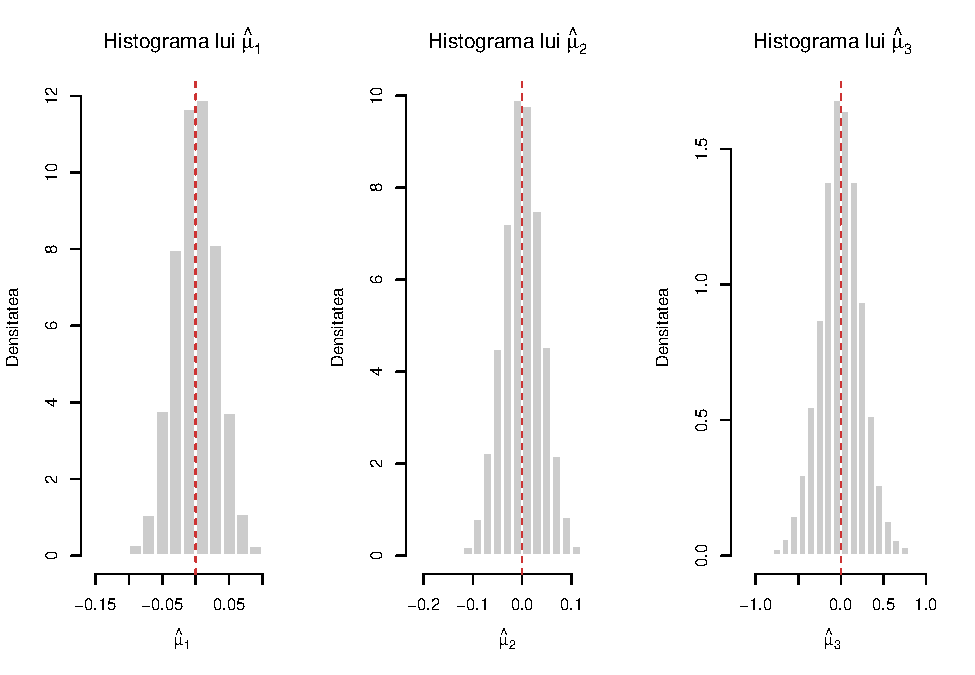
\includegraphics[width=0.7\linewidth]{Lab6_files/figure-latex/unnamed-chunk-5-1} \end{center}

\hypertarget{ilustrarea-consistenux21bei-unui-estimator}{%
\subsection{Ilustrarea consistenței unui
estimator}\label{ilustrarea-consistenux21bei-unui-estimator}}

\begin{rmdexercise}
Fie \(X_1,X_2,\ldots,X_n\) un eșantion de talie \(n\) dintr-o populație
\(Pois(\theta)\). Ilustrați grafic consistența estimatorului
\(\hat{\theta}_n = S_n^2\) trasând histograma repartiției lui
\(\hat{\theta}_n\) pentru \(n\in\{10,25,50,100\}\). Ce observați?
\end{rmdexercise}

Considerăm funcția \texttt{pois\_est} care pentru \(\theta\) fixat
simulează repartiția estimatorului \(\hat{\theta}_n\):

\begin{Shaded}
\begin{Highlighting}[]
\NormalTok{pois_est1 =}\StringTok{ }\ControlFlowTok{function}\NormalTok{(n, theta, S)\{}
  \CommentTok{# initializare}
\NormalTok{  sigma1 =}\StringTok{ }\KeywordTok{numeric}\NormalTok{(S)}
  
  \ControlFlowTok{for}\NormalTok{ (i }\ControlFlowTok{in} \DecValTok{1}\OperatorTok{:}\NormalTok{S)\{}
\NormalTok{    x =}\StringTok{ }\KeywordTok{rpois}\NormalTok{(n, theta)}
\NormalTok{    sigma1[i] =}\StringTok{ }\KeywordTok{var}\NormalTok{(x)}
\NormalTok{  \}}
  \CommentTok{# afisam varianta estimatorului}
  \KeywordTok{print}\NormalTok{(}\KeywordTok{paste0}\NormalTok{(}\StringTok{"Pentru n = "}\NormalTok{, n,}\StringTok{" varianta estimatorului este "}\NormalTok{, }\KeywordTok{var}\NormalTok{(sigma1)))}
  \KeywordTok{return}\NormalTok{(sigma1)}
\NormalTok{\}}
\end{Highlighting}
\end{Shaded}

Considerând \(\theta = 3\) și \(n\in\{10,25,50,100\}\) avem:

\begin{Shaded}
\begin{Highlighting}[]
\NormalTok{theta =}\StringTok{ }\DecValTok{3}

\KeywordTok{par}\NormalTok{(}\DataTypeTok{mfrow=}\KeywordTok{c}\NormalTok{(}\DecValTok{2}\NormalTok{,}\DecValTok{2}\NormalTok{))}
\NormalTok{a1 =}\StringTok{ }\KeywordTok{pois_est1}\NormalTok{(}\DecValTok{10}\NormalTok{, theta, }\DecValTok{50000}\NormalTok{)}
\NormalTok{[}\DecValTok{1}\NormalTok{] }\StringTok{"Pentru n = 10 varianta estimatorului este 2.30244438915425"}
\NormalTok{a2 =}\StringTok{ }\KeywordTok{pois_est1}\NormalTok{(}\DecValTok{25}\NormalTok{, theta, }\DecValTok{50000}\NormalTok{)}
\NormalTok{[}\DecValTok{1}\NormalTok{] }\StringTok{"Pentru n = 25 varianta estimatorului este 0.870906680642053"}
\NormalTok{a3 =}\StringTok{ }\KeywordTok{pois_est1}\NormalTok{(}\DecValTok{50}\NormalTok{, theta, }\DecValTok{50000}\NormalTok{)}
\NormalTok{[}\DecValTok{1}\NormalTok{] }\StringTok{"Pentru n = 50 varianta estimatorului este 0.428041768952562"}
\NormalTok{a4 =}\StringTok{ }\KeywordTok{pois_est1}\NormalTok{(}\DecValTok{100}\NormalTok{, theta, }\DecValTok{50000}\NormalTok{)}
\NormalTok{[}\DecValTok{1}\NormalTok{] }\StringTok{"Pentru n = 100 varianta estimatorului este 0.212316756387859"}


\KeywordTok{hist}\NormalTok{(a1, }\DataTypeTok{freq=}\OtherTok{FALSE}\NormalTok{, }\DataTypeTok{xlab=}\KeywordTok{expression}\NormalTok{(}\KeywordTok{hat}\NormalTok{(theta)[n]), }
     \DataTypeTok{col=}\StringTok{"gray80"}\NormalTok{, }\DataTypeTok{border=}\StringTok{"white"}\NormalTok{, }\DataTypeTok{main =} \StringTok{"n = 10"}\NormalTok{, }\DataTypeTok{xlim =} \KeywordTok{c}\NormalTok{(}\DecValTok{0}\NormalTok{,}\DecValTok{12}\NormalTok{),}
     \DataTypeTok{ylab =} \StringTok{"Densitatea"}\NormalTok{)}
\KeywordTok{abline}\NormalTok{(}\DataTypeTok{v=}\NormalTok{theta, }\DataTypeTok{col =} \StringTok{"brown3"}\NormalTok{, }\DataTypeTok{lty =} \DecValTok{2}\NormalTok{)}

\KeywordTok{hist}\NormalTok{(a2, }\DataTypeTok{freq=}\OtherTok{FALSE}\NormalTok{, }\DataTypeTok{xlab=}\KeywordTok{expression}\NormalTok{(}\KeywordTok{hat}\NormalTok{(theta)[n]), }
     \DataTypeTok{col=}\StringTok{"gray80"}\NormalTok{, }\DataTypeTok{border=}\StringTok{"white"}\NormalTok{, }\DataTypeTok{main =} \StringTok{"n = 25"}\NormalTok{, }\DataTypeTok{xlim =} \KeywordTok{c}\NormalTok{(}\DecValTok{0}\NormalTok{,}\DecValTok{12}\NormalTok{),}
     \DataTypeTok{ylab =} \StringTok{"Densitatea"}\NormalTok{)}
\KeywordTok{abline}\NormalTok{(}\DataTypeTok{v=}\NormalTok{theta, }\DataTypeTok{col =} \StringTok{"brown3"}\NormalTok{, }\DataTypeTok{lty =} \DecValTok{2}\NormalTok{)}

\KeywordTok{hist}\NormalTok{(a3, }\DataTypeTok{freq=}\OtherTok{FALSE}\NormalTok{, }\DataTypeTok{xlab=}\KeywordTok{expression}\NormalTok{(}\KeywordTok{hat}\NormalTok{(theta)[n]), }
     \DataTypeTok{col=}\StringTok{"gray80"}\NormalTok{, }\DataTypeTok{border=}\StringTok{"white"}\NormalTok{, }\DataTypeTok{main =} \StringTok{"n = 50"}\NormalTok{, }\DataTypeTok{xlim =} \KeywordTok{c}\NormalTok{(}\DecValTok{0}\NormalTok{,}\DecValTok{12}\NormalTok{),}
     \DataTypeTok{ylab =} \StringTok{"Densitatea"}\NormalTok{)}
\KeywordTok{abline}\NormalTok{(}\DataTypeTok{v=}\NormalTok{theta, }\DataTypeTok{col =} \StringTok{"brown3"}\NormalTok{, }\DataTypeTok{lty =} \DecValTok{2}\NormalTok{)}

\KeywordTok{hist}\NormalTok{(a4, }\DataTypeTok{freq=}\OtherTok{FALSE}\NormalTok{, }\DataTypeTok{xlab=}\KeywordTok{expression}\NormalTok{(}\KeywordTok{hat}\NormalTok{(theta)[n]), }
     \DataTypeTok{col=}\StringTok{"gray80"}\NormalTok{, }\DataTypeTok{border=}\StringTok{"white"}\NormalTok{, }\DataTypeTok{main =} \StringTok{"n = 100"}\NormalTok{, }\DataTypeTok{xlim =} \KeywordTok{c}\NormalTok{(}\DecValTok{0}\NormalTok{,}\DecValTok{12}\NormalTok{),}
     \DataTypeTok{ylab =} \StringTok{"Densitatea"}\NormalTok{)}
\KeywordTok{abline}\NormalTok{(}\DataTypeTok{v=}\NormalTok{theta, }\DataTypeTok{col =} \StringTok{"brown3"}\NormalTok{, }\DataTypeTok{lty =} \DecValTok{2}\NormalTok{)}
\end{Highlighting}
\end{Shaded}

\begin{center}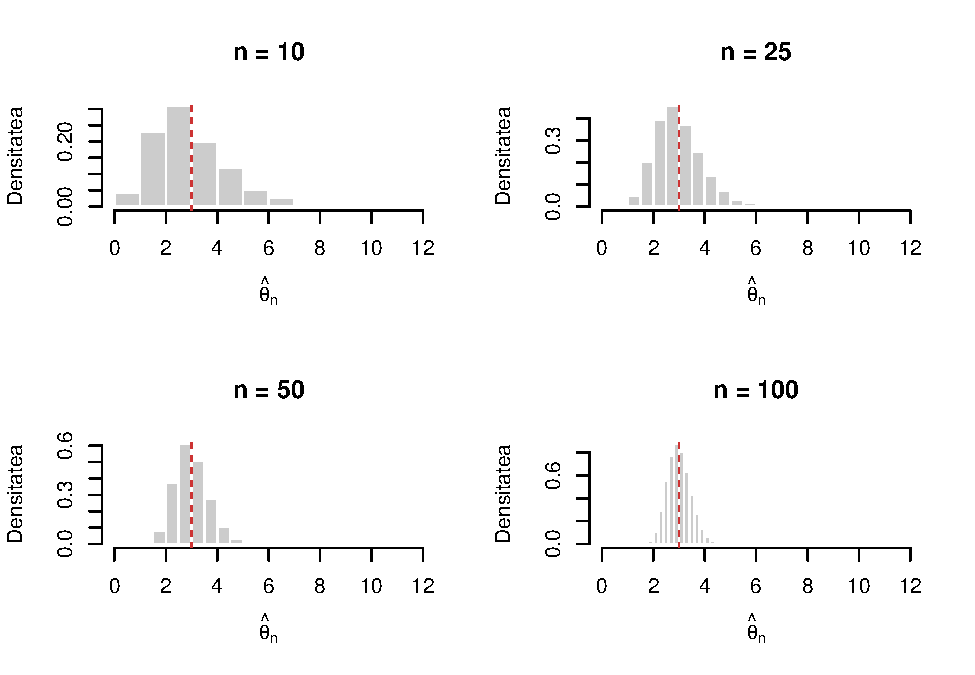
\includegraphics[width=0.7\linewidth]{Lab6_files/figure-latex/unnamed-chunk-8-1} \end{center}

Ce se întâmplă dacă în loc de \(\hat{\theta}_n\) considerăm estimatorul
\(\tilde{\theta}_n = \bar{X}_n\) sau estimatorul
\(\dot{\theta}_n = \sqrt{\bar{X}_n S_n^2}\) ?

Pentru \(\tilde{\theta}_n\) avem

\begin{Shaded}
\begin{Highlighting}[]
\NormalTok{pois_est2 =}\StringTok{ }\ControlFlowTok{function}\NormalTok{(n, theta, S)\{}
  \CommentTok{# initializare}
\NormalTok{  sigma2 =}\StringTok{ }\KeywordTok{numeric}\NormalTok{(S)}
  
  \ControlFlowTok{for}\NormalTok{ (i }\ControlFlowTok{in} \DecValTok{1}\OperatorTok{:}\NormalTok{S)\{}
\NormalTok{    x =}\StringTok{ }\KeywordTok{rpois}\NormalTok{(n, theta)}
\NormalTok{    sigma2[i] =}\StringTok{ }\KeywordTok{mean}\NormalTok{(x)}
\NormalTok{  \}}
  \CommentTok{# afisam varianta estimatorului}
  \KeywordTok{print}\NormalTok{(}\KeywordTok{paste0}\NormalTok{(}\StringTok{"Pentru n = "}\NormalTok{, n,}\StringTok{" varianta estimatorului este "}\NormalTok{, }\KeywordTok{var}\NormalTok{(sigma2)))}
  \KeywordTok{return}\NormalTok{(sigma2)}
\NormalTok{\}}

\NormalTok{theta =}\StringTok{ }\DecValTok{3}

\KeywordTok{par}\NormalTok{(}\DataTypeTok{mfrow=}\KeywordTok{c}\NormalTok{(}\DecValTok{2}\NormalTok{,}\DecValTok{2}\NormalTok{))}
\NormalTok{a1 =}\StringTok{ }\KeywordTok{pois_est2}\NormalTok{(}\DecValTok{10}\NormalTok{, theta, }\DecValTok{50000}\NormalTok{)}
\NormalTok{[}\DecValTok{1}\NormalTok{] }\StringTok{"Pentru n = 10 varianta estimatorului este 0.299715966123322"}
\NormalTok{a2 =}\StringTok{ }\KeywordTok{pois_est2}\NormalTok{(}\DecValTok{25}\NormalTok{, theta, }\DecValTok{50000}\NormalTok{)}
\NormalTok{[}\DecValTok{1}\NormalTok{] }\StringTok{"Pentru n = 25 varianta estimatorului este 0.121187195338147"}
\NormalTok{a3 =}\StringTok{ }\KeywordTok{pois_est2}\NormalTok{(}\DecValTok{50}\NormalTok{, theta, }\DecValTok{50000}\NormalTok{)}
\NormalTok{[}\DecValTok{1}\NormalTok{] }\StringTok{"Pentru n = 50 varianta estimatorului este 0.0600944942898858"}
\NormalTok{a4 =}\StringTok{ }\KeywordTok{pois_est2}\NormalTok{(}\DecValTok{100}\NormalTok{, theta, }\DecValTok{50000}\NormalTok{)}
\NormalTok{[}\DecValTok{1}\NormalTok{] }\StringTok{"Pentru n = 100 varianta estimatorului este 0.0300141779183984"}


\KeywordTok{hist}\NormalTok{(a1, }\DataTypeTok{freq=}\OtherTok{FALSE}\NormalTok{, }\DataTypeTok{xlab=}\KeywordTok{expression}\NormalTok{(}\KeywordTok{tilde}\NormalTok{(theta)[n]), }
     \DataTypeTok{col=}\StringTok{"gray80"}\NormalTok{, }\DataTypeTok{border=}\StringTok{"white"}\NormalTok{, }\DataTypeTok{main =} \StringTok{"n = 10"}\NormalTok{, }\DataTypeTok{xlim =} \KeywordTok{c}\NormalTok{(}\DecValTok{0}\NormalTok{,}\DecValTok{12}\NormalTok{),}
     \DataTypeTok{ylab =} \StringTok{"Densitatea"}\NormalTok{)}
\KeywordTok{abline}\NormalTok{(}\DataTypeTok{v=}\NormalTok{theta, }\DataTypeTok{col =} \StringTok{"brown3"}\NormalTok{, }\DataTypeTok{lty =} \DecValTok{2}\NormalTok{)}

\KeywordTok{hist}\NormalTok{(a2, }\DataTypeTok{freq=}\OtherTok{FALSE}\NormalTok{, }\DataTypeTok{xlab=}\KeywordTok{expression}\NormalTok{(}\KeywordTok{tilde}\NormalTok{(theta)[n]), }
     \DataTypeTok{col=}\StringTok{"gray80"}\NormalTok{, }\DataTypeTok{border=}\StringTok{"white"}\NormalTok{, }\DataTypeTok{main =} \StringTok{"n = 25"}\NormalTok{, }\DataTypeTok{xlim =} \KeywordTok{c}\NormalTok{(}\DecValTok{0}\NormalTok{,}\DecValTok{12}\NormalTok{),}
     \DataTypeTok{ylab =} \StringTok{"Densitatea"}\NormalTok{)}
\KeywordTok{abline}\NormalTok{(}\DataTypeTok{v=}\NormalTok{theta, }\DataTypeTok{col =} \StringTok{"brown3"}\NormalTok{, }\DataTypeTok{lty =} \DecValTok{2}\NormalTok{)}

\KeywordTok{hist}\NormalTok{(a3, }\DataTypeTok{freq=}\OtherTok{FALSE}\NormalTok{, }\DataTypeTok{xlab=}\KeywordTok{expression}\NormalTok{(}\KeywordTok{tilde}\NormalTok{(theta)[n]), }
     \DataTypeTok{col=}\StringTok{"gray80"}\NormalTok{, }\DataTypeTok{border=}\StringTok{"white"}\NormalTok{, }\DataTypeTok{main =} \StringTok{"n = 50"}\NormalTok{, }\DataTypeTok{xlim =} \KeywordTok{c}\NormalTok{(}\DecValTok{0}\NormalTok{,}\DecValTok{12}\NormalTok{),}
     \DataTypeTok{ylab =} \StringTok{"Densitatea"}\NormalTok{)}
\KeywordTok{abline}\NormalTok{(}\DataTypeTok{v=}\NormalTok{theta, }\DataTypeTok{col =} \StringTok{"brown3"}\NormalTok{, }\DataTypeTok{lty =} \DecValTok{2}\NormalTok{)}

\KeywordTok{hist}\NormalTok{(a4, }\DataTypeTok{freq=}\OtherTok{FALSE}\NormalTok{, }\DataTypeTok{xlab=}\KeywordTok{expression}\NormalTok{(}\KeywordTok{tilde}\NormalTok{(theta)[n]), }
     \DataTypeTok{col=}\StringTok{"gray80"}\NormalTok{, }\DataTypeTok{border=}\StringTok{"white"}\NormalTok{, }\DataTypeTok{main =} \StringTok{"n = 100"}\NormalTok{, }\DataTypeTok{xlim =} \KeywordTok{c}\NormalTok{(}\DecValTok{0}\NormalTok{,}\DecValTok{12}\NormalTok{),}
     \DataTypeTok{ylab =} \StringTok{"Densitatea"}\NormalTok{)}
\KeywordTok{abline}\NormalTok{(}\DataTypeTok{v=}\NormalTok{theta, }\DataTypeTok{col =} \StringTok{"brown3"}\NormalTok{, }\DataTypeTok{lty =} \DecValTok{2}\NormalTok{)}
\end{Highlighting}
\end{Shaded}

\begin{center}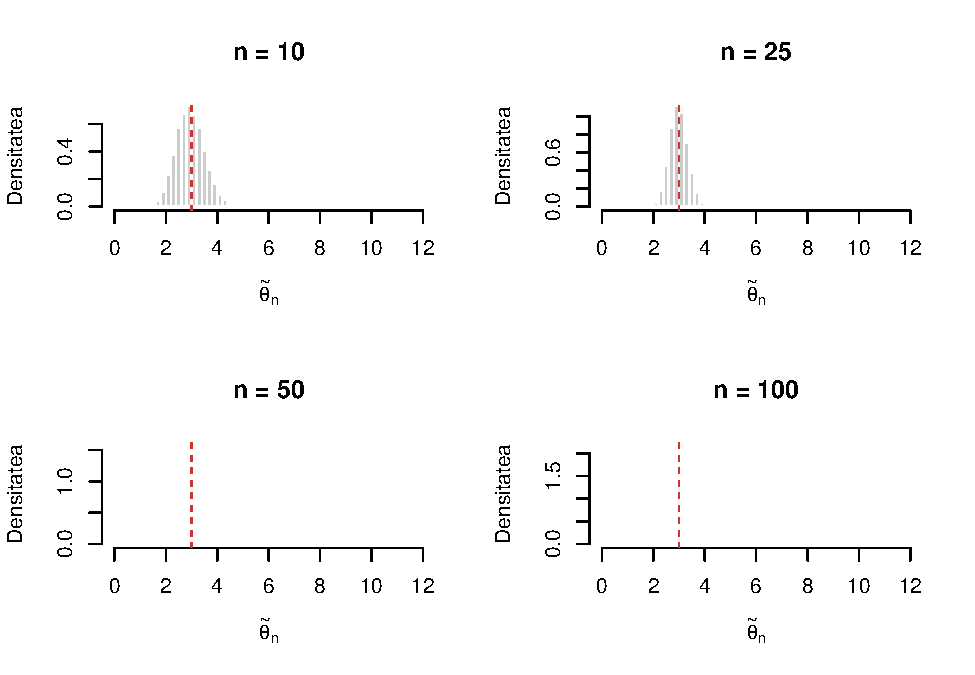
\includegraphics[width=0.7\linewidth]{Lab6_files/figure-latex/unnamed-chunk-9-1} \end{center}

iar pentru \(\dot{\theta}_n\) avem

\begin{Shaded}
\begin{Highlighting}[]
\NormalTok{pois_est3 =}\StringTok{ }\ControlFlowTok{function}\NormalTok{(n, theta, S)\{}
  \CommentTok{# initializare}
\NormalTok{  sigma3 =}\StringTok{ }\KeywordTok{numeric}\NormalTok{(S)}
  
  \ControlFlowTok{for}\NormalTok{ (i }\ControlFlowTok{in} \DecValTok{1}\OperatorTok{:}\NormalTok{S)\{}
\NormalTok{    x =}\StringTok{ }\KeywordTok{rpois}\NormalTok{(n, theta)}
\NormalTok{    sigma3[i] =}\StringTok{ }\KeywordTok{sqrt}\NormalTok{(}\KeywordTok{mean}\NormalTok{(x)}\OperatorTok{*}\KeywordTok{var}\NormalTok{(x))}
\NormalTok{  \}}
  \CommentTok{# afisam varianta estimatorului}
  \KeywordTok{print}\NormalTok{(}\KeywordTok{paste0}\NormalTok{(}\StringTok{"Pentru n = "}\NormalTok{, n,}\StringTok{" varianta estimatorului este "}\NormalTok{, }\KeywordTok{var}\NormalTok{(sigma3)))}
  \KeywordTok{return}\NormalTok{(sigma3)}
\NormalTok{\}}

\NormalTok{theta =}\StringTok{ }\DecValTok{3}

\KeywordTok{par}\NormalTok{(}\DataTypeTok{mfrow=}\KeywordTok{c}\NormalTok{(}\DecValTok{2}\NormalTok{,}\DecValTok{2}\NormalTok{))}

\NormalTok{a1 =}\StringTok{ }\KeywordTok{pois_est3}\NormalTok{(}\DecValTok{10}\NormalTok{, theta, }\DecValTok{50000}\NormalTok{)}
\NormalTok{[}\DecValTok{1}\NormalTok{] }\StringTok{"Pentru n = 10 varianta estimatorului este 0.774312512559173"}
\NormalTok{a2 =}\StringTok{ }\KeywordTok{pois_est3}\NormalTok{(}\DecValTok{25}\NormalTok{, theta, }\DecValTok{50000}\NormalTok{)}
\NormalTok{[}\DecValTok{1}\NormalTok{] }\StringTok{"Pentru n = 25 varianta estimatorului este 0.300199856748503"}
\NormalTok{a3 =}\StringTok{ }\KeywordTok{pois_est3}\NormalTok{(}\DecValTok{50}\NormalTok{, theta, }\DecValTok{50000}\NormalTok{)}
\NormalTok{[}\DecValTok{1}\NormalTok{] }\StringTok{"Pentru n = 50 varianta estimatorului este 0.151213574285"}
\NormalTok{a4 =}\StringTok{ }\KeywordTok{pois_est3}\NormalTok{(}\DecValTok{100}\NormalTok{, theta, }\DecValTok{50000}\NormalTok{)}
\NormalTok{[}\DecValTok{1}\NormalTok{] }\StringTok{"Pentru n = 100 varianta estimatorului este 0.0752523336106622"}


\KeywordTok{hist}\NormalTok{(a1, }\DataTypeTok{freq=}\OtherTok{FALSE}\NormalTok{, }\DataTypeTok{xlab=}\KeywordTok{expression}\NormalTok{(}\KeywordTok{dot}\NormalTok{(theta)[n]), }
     \DataTypeTok{col=}\StringTok{"gray80"}\NormalTok{, }\DataTypeTok{border=}\StringTok{"white"}\NormalTok{, }\DataTypeTok{main =} \StringTok{"n = 10"}\NormalTok{, }\DataTypeTok{xlim =} \KeywordTok{c}\NormalTok{(}\DecValTok{0}\NormalTok{,}\DecValTok{12}\NormalTok{),}
     \DataTypeTok{ylab =} \StringTok{"Densitatea"}\NormalTok{)}
\KeywordTok{abline}\NormalTok{(}\DataTypeTok{v=}\NormalTok{theta, }\DataTypeTok{col =} \StringTok{"brown3"}\NormalTok{, }\DataTypeTok{lty =} \DecValTok{2}\NormalTok{)}

\KeywordTok{hist}\NormalTok{(a2, }\DataTypeTok{freq=}\OtherTok{FALSE}\NormalTok{, }\DataTypeTok{xlab=}\KeywordTok{expression}\NormalTok{(}\KeywordTok{dot}\NormalTok{(theta)[n]), }
     \DataTypeTok{col=}\StringTok{"gray80"}\NormalTok{, }\DataTypeTok{border=}\StringTok{"white"}\NormalTok{, }\DataTypeTok{main =} \StringTok{"n = 25"}\NormalTok{, }\DataTypeTok{xlim =} \KeywordTok{c}\NormalTok{(}\DecValTok{0}\NormalTok{,}\DecValTok{12}\NormalTok{),}
     \DataTypeTok{ylab =} \StringTok{"Densitatea"}\NormalTok{)}
\KeywordTok{abline}\NormalTok{(}\DataTypeTok{v=}\NormalTok{theta, }\DataTypeTok{col =} \StringTok{"brown3"}\NormalTok{, }\DataTypeTok{lty =} \DecValTok{2}\NormalTok{)}

\KeywordTok{hist}\NormalTok{(a3, }\DataTypeTok{freq=}\OtherTok{FALSE}\NormalTok{, }\DataTypeTok{xlab=}\KeywordTok{expression}\NormalTok{(}\KeywordTok{dot}\NormalTok{(theta)[n]), }
     \DataTypeTok{col=}\StringTok{"gray80"}\NormalTok{, }\DataTypeTok{border=}\StringTok{"white"}\NormalTok{, }\DataTypeTok{main =} \StringTok{"n = 50"}\NormalTok{, }\DataTypeTok{xlim =} \KeywordTok{c}\NormalTok{(}\DecValTok{0}\NormalTok{,}\DecValTok{12}\NormalTok{),}
     \DataTypeTok{ylab =} \StringTok{"Densitatea"}\NormalTok{)}
\KeywordTok{abline}\NormalTok{(}\DataTypeTok{v=}\NormalTok{theta, }\DataTypeTok{col =} \StringTok{"brown3"}\NormalTok{, }\DataTypeTok{lty =} \DecValTok{2}\NormalTok{)}

\KeywordTok{hist}\NormalTok{(a4, }\DataTypeTok{freq=}\OtherTok{FALSE}\NormalTok{, }\DataTypeTok{xlab=}\KeywordTok{expression}\NormalTok{(}\KeywordTok{dot}\NormalTok{(theta)[n]), }
     \DataTypeTok{col=}\StringTok{"gray80"}\NormalTok{, }\DataTypeTok{border=}\StringTok{"white"}\NormalTok{, }\DataTypeTok{main =} \StringTok{"n = 100"}\NormalTok{, }\DataTypeTok{xlim =} \KeywordTok{c}\NormalTok{(}\DecValTok{0}\NormalTok{,}\DecValTok{12}\NormalTok{),}
     \DataTypeTok{ylab =} \StringTok{"Densitatea"}\NormalTok{)}
\KeywordTok{abline}\NormalTok{(}\DataTypeTok{v=}\NormalTok{theta, }\DataTypeTok{col =} \StringTok{"brown3"}\NormalTok{, }\DataTypeTok{lty =} \DecValTok{2}\NormalTok{)}
\end{Highlighting}
\end{Shaded}

\begin{center}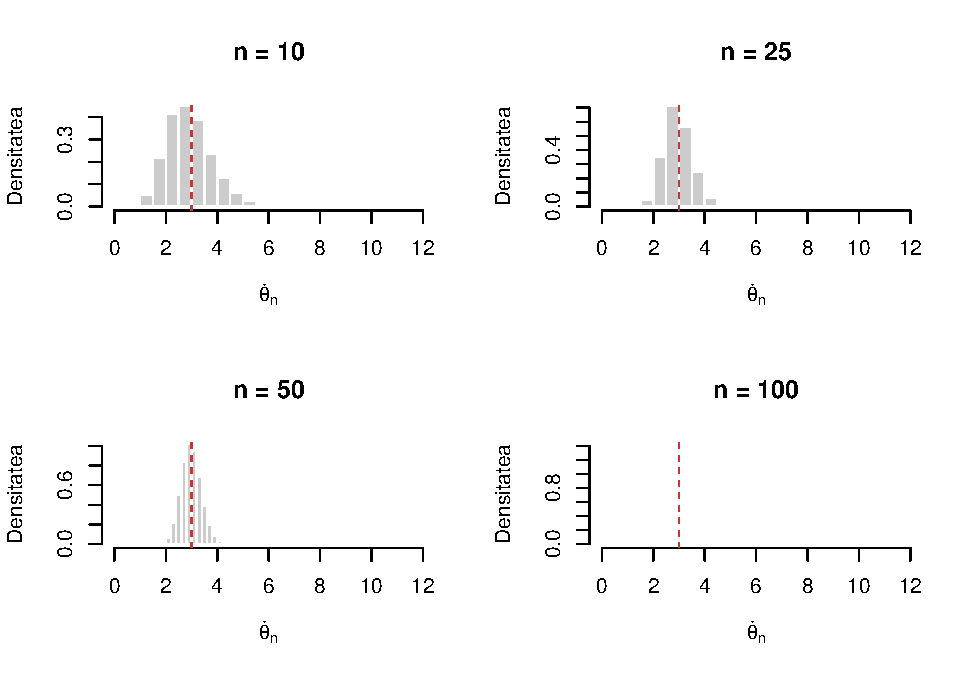
\includegraphics[width=0.7\linewidth]{Lab6_files/figure-latex/unnamed-chunk-10-1} \end{center}

\hypertarget{estimare-prin-metoda-verosimilitux103ux21bii-maxime}{%
\section{Estimare prin metoda verosimilității
maxime}\label{estimare-prin-metoda-verosimilitux103ux21bii-maxime}}

\hypertarget{exemplu-evm-nu-este-uxeentotdeauna-media-eux219antionului-chiar-dacux103-mathbbe_thetahattheta_n-theta}{%
\subsection{\texorpdfstring{Exemplu: EVM nu este întotdeauna media
eșantionului chiar dacă
\(\mathbb{E}_{\theta}[\hat{\theta}_n] = \theta\)}{Exemplu: EVM nu este întotdeauna media eșantionului chiar dacă \textbackslash mathbb\{E\}\_\{\textbackslash theta\}{[}\textbackslash hat\{\textbackslash theta\}\_n{]} = \textbackslash theta}}\label{exemplu-evm-nu-este-uxeentotdeauna-media-eux219antionului-chiar-dacux103-mathbbe_thetahattheta_n-theta}}

\begin{rmdexercise}
Fie \(X_1,X_2,\ldots,X_n\) un eșantion de talie \(n\) dintr-o populație
Laplace \(L(\theta, c)\) a cărei densitate este dată de formula

\[
  f_{\theta, c}(x) = \frac{1}{2c}e^{-\frac{|x-\theta|}{c}}, \quad -\infty<x<\infty
\]

\begin{enumerate}
\def\labelenumi{\alph{enumi})}
\item
  Ilustrați grafic densitatea și funcția de repartiție a repartiției
  Laplace pentru diferite valori ale parametrilor \(\theta\) (de
  locație) și \(c\) (de scală), e.g.~\(\theta\in\{0, 3\}\) și
  \(c\in\{1,2,3,4\}\).
\item
  Determinați estimatorul de verosimilitate maximă \(\hat{\theta}_n\)
  pentru \(\theta\).
\end{enumerate}
\end{rmdexercise}

\begin{enumerate}
\def\labelenumi{\alph{enumi})}
\tightlist
\item
  Se poate arăta cu ușurință că funcția de repartiție a repartiției
  Laplace \(L(\theta, c)\) este
\end{enumerate}

\[
  F_{\theta, c}(x) = \frac{1}{2} + \frac{1}{2}\operatorname{sgn}(x-\theta)\left(1-e^{-\frac{|x-\theta|}{c}}\right) = \left\{\begin{array}{ll}
    \frac{1}{2}e^{-\frac{|x-\theta|}{c}}, & x<\theta\\
    1-\frac{1}{2}e^{-\frac{|x-\theta|}{c}}, & x\geq\theta
  \end{array}\right.
\]

Ilustrarea grafică a densității și a funcției de repartiție pentru
repartiția Laplace:

\begin{Shaded}
\begin{Highlighting}[]
\CommentTok{# Cream functia de densitate si de repartitie }

\NormalTok{dLaplace =}\StringTok{ }\ControlFlowTok{function}\NormalTok{ (x, }\DataTypeTok{mu =} \DecValTok{0}\NormalTok{, }\DataTypeTok{b =} \DecValTok{1}\NormalTok{) }
\NormalTok{\{}
\NormalTok{    d <-}\StringTok{ }\KeywordTok{exp}\NormalTok{(}\OperatorTok{-}\KeywordTok{abs}\NormalTok{(x }\OperatorTok{-}\StringTok{ }\NormalTok{mu)}\OperatorTok{/}\NormalTok{b)}\OperatorTok{/}\NormalTok{(}\DecValTok{2} \OperatorTok{*}\StringTok{ }\NormalTok{b)}
    \KeywordTok{return}\NormalTok{(d)}
\NormalTok{\}}

\NormalTok{pLaplace =}\StringTok{ }\ControlFlowTok{function}\NormalTok{ (q, }\DataTypeTok{mu =} \DecValTok{0}\NormalTok{, }\DataTypeTok{b =} \DecValTok{1}\NormalTok{) }
\NormalTok{\{}
\NormalTok{    x <-}\StringTok{ }\NormalTok{q }\OperatorTok{-}\StringTok{ }\NormalTok{mu}
    \FloatTok{0.5} \OperatorTok{+}\StringTok{ }\FloatTok{0.5} \OperatorTok{*}\StringTok{ }\KeywordTok{sign}\NormalTok{(x) }\OperatorTok{*}\StringTok{ }\NormalTok{(}\DecValTok{1} \OperatorTok{-}\StringTok{ }\KeywordTok{exp}\NormalTok{(}\OperatorTok{-}\KeywordTok{abs}\NormalTok{(x)}\OperatorTok{/}\NormalTok{b))}
\NormalTok{\}}

\CommentTok{# Generam graficele }
\NormalTok{pars =}\StringTok{ }\KeywordTok{matrix}\NormalTok{(}\KeywordTok{c}\NormalTok{(}\DecValTok{0}\NormalTok{, }\DecValTok{1}\NormalTok{, }\DecValTok{0}\NormalTok{, }\DecValTok{2}\NormalTok{, }\DecValTok{0}\NormalTok{, }\DecValTok{3}\NormalTok{, }\DecValTok{0}\NormalTok{, }\DecValTok{4}\NormalTok{, }\DecValTok{3}\NormalTok{, }\DecValTok{1}\NormalTok{, }\DecValTok{3}\NormalTok{, }\DecValTok{3}\NormalTok{, }\DecValTok{3}\NormalTok{, }\DecValTok{4}\NormalTok{), }
              \DataTypeTok{ncol =} \DecValTok{2}\NormalTok{, }\DataTypeTok{byrow =} \OtherTok{TRUE}\NormalTok{)}

\NormalTok{x =}\StringTok{ }\KeywordTok{seq}\NormalTok{(}\OperatorTok{-}\DecValTok{8}\NormalTok{, }\DecValTok{8}\NormalTok{, }\DataTypeTok{length.out =} \DecValTok{250}\NormalTok{)}

\KeywordTok{set.seed}\NormalTok{(}\DecValTok{1234}\NormalTok{)}
\NormalTok{cols =}\StringTok{ }\KeywordTok{sample}\NormalTok{(}\KeywordTok{colors}\NormalTok{(), }\KeywordTok{nrow}\NormalTok{(pars))}

\KeywordTok{par}\NormalTok{(}\DataTypeTok{mfrow =} \KeywordTok{c}\NormalTok{(}\DecValTok{1}\NormalTok{, }\DecValTok{2}\NormalTok{))}
\CommentTok{# densitatile}
\KeywordTok{plot}\NormalTok{(x, }\KeywordTok{dLaplace}\NormalTok{(x, }\DataTypeTok{mu =}\NormalTok{ pars[}\DecValTok{1}\NormalTok{, }\DecValTok{1}\NormalTok{], }\DataTypeTok{b =}\NormalTok{ pars[}\DecValTok{1}\NormalTok{, }\DecValTok{2}\NormalTok{]),}
     \DataTypeTok{xlab =} \StringTok{"x"}\NormalTok{,}
     \DataTypeTok{ylab =} \KeywordTok{TeX}\NormalTok{(}\StringTok{"$f_\{}\CharTok{\textbackslash{}\textbackslash{}}\StringTok{theta, c\}(x)$"}\NormalTok{),}
     \DataTypeTok{ylim =} \KeywordTok{c}\NormalTok{(}\DecValTok{0}\NormalTok{,}\DecValTok{1}\NormalTok{),}
     \DataTypeTok{col =} \StringTok{"brown3"}\NormalTok{, }
     \DataTypeTok{lwd =} \DecValTok{2}\NormalTok{, }\DataTypeTok{type =} \StringTok{"l"}\NormalTok{,}
     \DataTypeTok{bty =} \StringTok{"n"}\NormalTok{,}
     \DataTypeTok{main =} \StringTok{"Densitatea"}\NormalTok{)}

\ControlFlowTok{for}\NormalTok{ (i }\ControlFlowTok{in} \KeywordTok{seq}\NormalTok{(}\KeywordTok{nrow}\NormalTok{(pars)}\OperatorTok{-}\DecValTok{1}\NormalTok{))\{}
\NormalTok{  mu =}\StringTok{ }\NormalTok{pars[i}\OperatorTok{+}\DecValTok{1}\NormalTok{, }\DecValTok{1}\NormalTok{]}
\NormalTok{  b =}\StringTok{ }\NormalTok{pars[i}\OperatorTok{+}\DecValTok{1}\NormalTok{, }\DecValTok{2}\NormalTok{]}
    
\NormalTok{  y =}\StringTok{ }\KeywordTok{dLaplace}\NormalTok{(x, }\DataTypeTok{mu =}\NormalTok{ mu, }\DataTypeTok{b =}\NormalTok{ b)}
  
  \KeywordTok{lines}\NormalTok{(x, y, }\DataTypeTok{lwd =} \DecValTok{2}\NormalTok{, }
        \DataTypeTok{col =}\NormalTok{ cols[i])}
\NormalTok{\}}

\KeywordTok{legend}\NormalTok{(}\StringTok{"topright"}\NormalTok{, }
       \DataTypeTok{legend =} \KeywordTok{TeX}\NormalTok{(}\KeywordTok{paste0}\NormalTok{(}\StringTok{"$}\CharTok{\textbackslash{}\textbackslash{}}\StringTok{theta = "}\NormalTok{, pars[,}\DecValTok{1}\NormalTok{], }\StringTok{", }\CharTok{\textbackslash{}\textbackslash{}}\StringTok{c = "}\NormalTok{, pars[,}\DecValTok{2}\NormalTok{], }\StringTok{"$"}\NormalTok{)),}
       \DataTypeTok{col =}\NormalTok{ cols,}
       \DataTypeTok{lwd =} \KeywordTok{rep}\NormalTok{(}\DecValTok{2}\NormalTok{, }\KeywordTok{nrow}\NormalTok{(pars)),}
       \DataTypeTok{bty =} \StringTok{"n"}\NormalTok{,}
       \DataTypeTok{cex =} \FloatTok{0.7}\NormalTok{,}
       \DataTypeTok{seg.len =} \FloatTok{1.5}\NormalTok{)}

\CommentTok{# functiile de repartitie}
\KeywordTok{plot}\NormalTok{(x, }\KeywordTok{pLaplace}\NormalTok{(x, }\DataTypeTok{mu =}\NormalTok{ pars[}\DecValTok{1}\NormalTok{, }\DecValTok{1}\NormalTok{], }\DataTypeTok{b =}\NormalTok{ pars[}\DecValTok{1}\NormalTok{, }\DecValTok{2}\NormalTok{]),}
     \DataTypeTok{xlab =} \StringTok{"x"}\NormalTok{,}
     \DataTypeTok{ylab =} \KeywordTok{TeX}\NormalTok{(}\StringTok{"$F_\{}\CharTok{\textbackslash{}\textbackslash{}}\StringTok{theta, c\}(x)$"}\NormalTok{),}
     \DataTypeTok{ylim =} \KeywordTok{c}\NormalTok{(}\DecValTok{0}\NormalTok{,}\DecValTok{1}\NormalTok{),}
     \DataTypeTok{col =} \StringTok{"brown3"}\NormalTok{, }
     \DataTypeTok{lwd =} \DecValTok{2}\NormalTok{, }\DataTypeTok{type =} \StringTok{"l"}\NormalTok{,}
     \DataTypeTok{bty =} \StringTok{"n"}\NormalTok{,}
     \DataTypeTok{main =} \StringTok{"Functia de repartitie"}\NormalTok{)}

\ControlFlowTok{for}\NormalTok{ (i }\ControlFlowTok{in} \KeywordTok{seq}\NormalTok{(}\KeywordTok{nrow}\NormalTok{(pars)}\OperatorTok{-}\DecValTok{1}\NormalTok{))\{}
\NormalTok{  mu =}\StringTok{ }\NormalTok{pars[i}\OperatorTok{+}\DecValTok{1}\NormalTok{, }\DecValTok{1}\NormalTok{]}
\NormalTok{  b =}\StringTok{ }\NormalTok{pars[i}\OperatorTok{+}\DecValTok{1}\NormalTok{, }\DecValTok{2}\NormalTok{]}
  
\NormalTok{  y =}\StringTok{ }\KeywordTok{pLaplace}\NormalTok{(x, }\DataTypeTok{mu =}\NormalTok{ mu, }\DataTypeTok{b =}\NormalTok{ b)}
  
  \KeywordTok{lines}\NormalTok{(x, y, }\DataTypeTok{lwd =} \DecValTok{2}\NormalTok{, }
        \DataTypeTok{col =}\NormalTok{ cols[i])}
\NormalTok{\}}

\KeywordTok{legend}\NormalTok{(}\StringTok{"bottomright"}\NormalTok{, }
       \DataTypeTok{legend =} \KeywordTok{TeX}\NormalTok{(}\KeywordTok{paste0}\NormalTok{(}\StringTok{"$}\CharTok{\textbackslash{}\textbackslash{}}\StringTok{theta = "}\NormalTok{, pars[,}\DecValTok{1}\NormalTok{], }\StringTok{", }\CharTok{\textbackslash{}\textbackslash{}}\StringTok{c = "}\NormalTok{, pars[,}\DecValTok{2}\NormalTok{], }\StringTok{"$"}\NormalTok{)),}
       \DataTypeTok{col =}\NormalTok{ cols,}
       \DataTypeTok{lwd =} \KeywordTok{rep}\NormalTok{(}\DecValTok{2}\NormalTok{, }\KeywordTok{nrow}\NormalTok{(pars)),}
       \DataTypeTok{bty =} \StringTok{"n"}\NormalTok{,}
       \DataTypeTok{cex =} \FloatTok{0.7}\NormalTok{,}
       \DataTypeTok{seg.len =} \FloatTok{1.5}\NormalTok{)}
\end{Highlighting}
\end{Shaded}

\begin{center}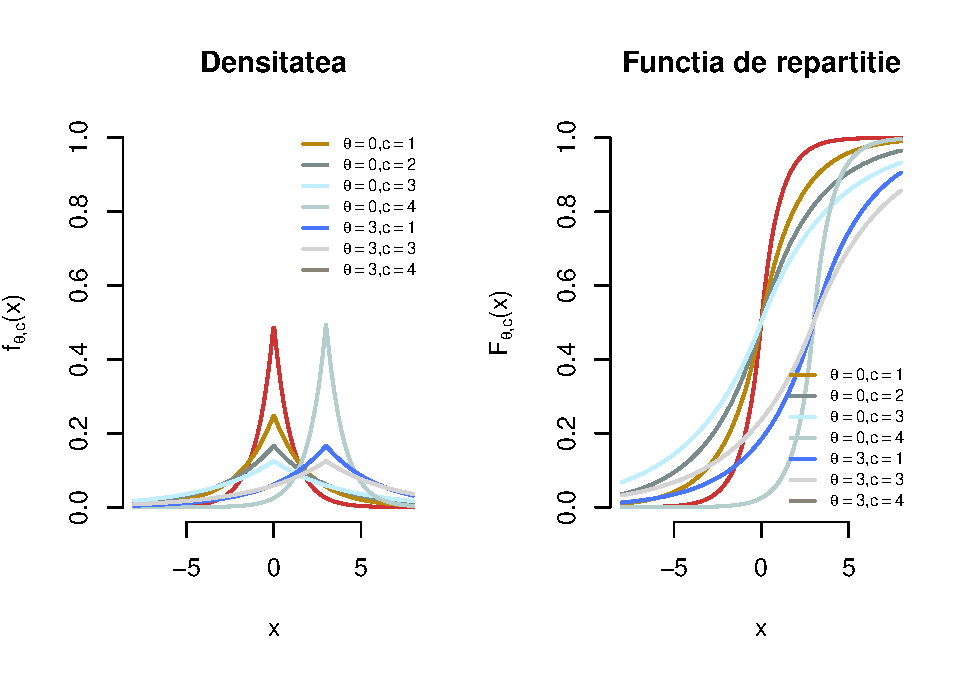
\includegraphics[width=0.7\linewidth]{Lab6_files/figure-latex/unnamed-chunk-12-1} \end{center}

\begin{enumerate}
\def\labelenumi{\alph{enumi})}
\setcounter{enumi}{1}
\tightlist
\item
  Pentru a determina estimatorul de verosimilitate maximă să observăm că
  funcția de verosimilitate este
\end{enumerate}

\[
L(\theta|\mathbf{X}) = \prod_{i=1}^{n}\left(\frac{1}{2c}e^{-\frac{|X_i-\theta|}{c}}\right) = \frac{1}{(2c)^n}e^{-\sum_{i=1}^{n}\frac{|X_i-\theta|}{c}}
\]

și acesta ia valoarea maximă pentru toate valorile lui \(\theta\) care
minimizează funcția de la exponent

\[
  M(\theta) = \sum_{i=1}^{n}|X_i-\theta| = \sum_{i=1}^{n}|X_{(i)}-\theta|,
\]

unde \(x_{(i)}\) este statistica de ordine de rang \(i\). Se poate vedea
că funcția \(M(\theta)\) este continuă și afină pe porțiuni din figura
de mai jos (pentru un eșantion de talie \(10\) dintr-o populație
\(L(3,1)\) - creați o funcție care vă permite să generați observații
repartizate Laplace).

\begin{Shaded}
\begin{Highlighting}[]
\NormalTok{rLaplace =}\StringTok{ }\ControlFlowTok{function}\NormalTok{ (n, }\DataTypeTok{mu =} \DecValTok{0}\NormalTok{, }\DataTypeTok{b =} \DecValTok{1}\NormalTok{) }
\NormalTok{\{}
\NormalTok{    u <-}\StringTok{ }\KeywordTok{runif}\NormalTok{(n) }\OperatorTok{-}\StringTok{ }\FloatTok{0.5}
\NormalTok{    x <-}\StringTok{ }\NormalTok{mu }\OperatorTok{-}\StringTok{ }\NormalTok{b }\OperatorTok{*}\StringTok{ }\KeywordTok{sign}\NormalTok{(u) }\OperatorTok{*}\StringTok{ }\KeywordTok{log}\NormalTok{(}\DecValTok{1} \OperatorTok{-}\StringTok{ }\DecValTok{2} \OperatorTok{*}\StringTok{ }\KeywordTok{abs}\NormalTok{(u))}
    \KeywordTok{return}\NormalTok{(x)}
\NormalTok{\}}

\NormalTok{theta0 =}\StringTok{ }\DecValTok{3}
\NormalTok{b =}\StringTok{ }\DecValTok{1}

\KeywordTok{set.seed}\NormalTok{(}\DecValTok{333}\NormalTok{)}
\NormalTok{x =}\StringTok{ }\KeywordTok{rLaplace}\NormalTok{(}\DecValTok{10}\NormalTok{, }\DataTypeTok{mu =}\NormalTok{ theta0, }\DataTypeTok{b =}\NormalTok{ b)}

\NormalTok{M_theta =}\StringTok{ }\ControlFlowTok{function}\NormalTok{(x, theta)\{}
  \KeywordTok{sapply}\NormalTok{(theta, }\ControlFlowTok{function}\NormalTok{(t)\{}\KeywordTok{sum}\NormalTok{(}\KeywordTok{abs}\NormalTok{(x}\OperatorTok{-}\NormalTok{t))\})}
\NormalTok{\}}

\NormalTok{theta =}\StringTok{ }\KeywordTok{seq}\NormalTok{(}\KeywordTok{min}\NormalTok{(x), }\KeywordTok{max}\NormalTok{(x), }\DataTypeTok{length.out =} \DecValTok{500}\NormalTok{)}
\NormalTok{M =}\StringTok{ }\KeywordTok{M_theta}\NormalTok{(x, theta)}

\KeywordTok{plot}\NormalTok{(theta, M, }\DataTypeTok{type =} \StringTok{"l"}\NormalTok{, }
     \DataTypeTok{xlab =} \KeywordTok{TeX}\NormalTok{(}\StringTok{"$}\CharTok{\textbackslash{}\textbackslash{}}\StringTok{theta$"}\NormalTok{),}
     \DataTypeTok{ylab =} \KeywordTok{TeX}\NormalTok{(}\StringTok{"$M(}\CharTok{\textbackslash{}\textbackslash{}}\StringTok{theta)$"}\NormalTok{),}
     \DataTypeTok{bty =} \StringTok{"n"}\NormalTok{, }\DataTypeTok{lwd =} \DecValTok{2}\NormalTok{,}
     \DataTypeTok{col =} \StringTok{"royalblue"}\NormalTok{)}
\end{Highlighting}
\end{Shaded}

\begin{center}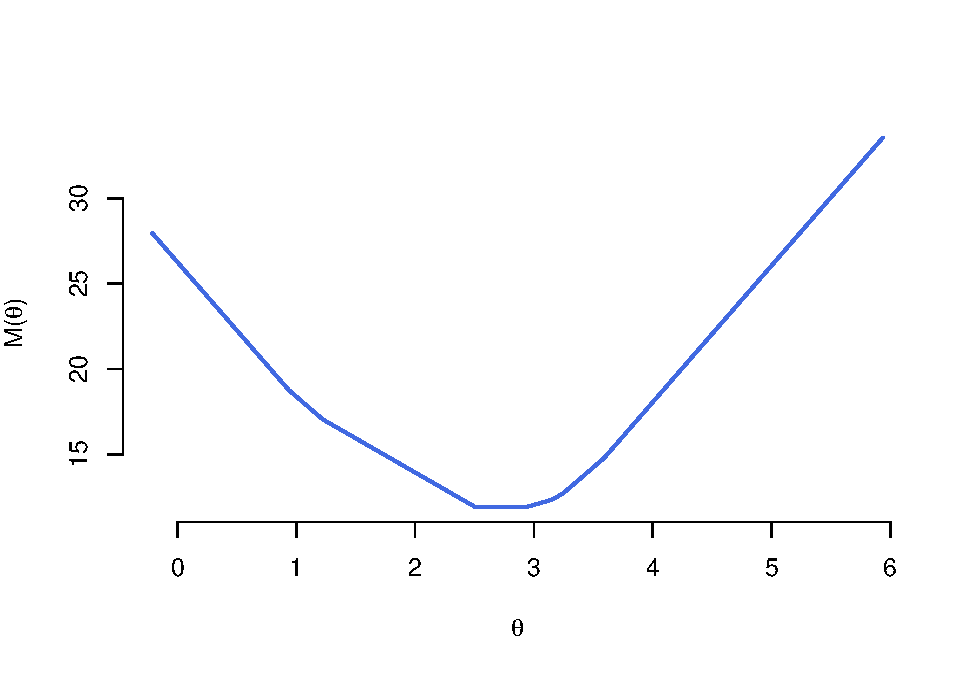
\includegraphics[width=0.7\linewidth]{Lab6_files/figure-latex/unnamed-chunk-13-1} \end{center}

Observăm că dacă \(\theta\) se află între statistica de ordine de rang
\(m\) și cea de rang \(m+1\), i.e.~\(X_{(m)}\leq \theta\leq X_{(m+1)}\),
atunci am avea că \(X_{(i)} \leq X_{(m)} \leq \theta\) dacă \(i\leq m\)
și \(\theta\leq X_{(m+1)}\leq X_{(i)}\) dacă \(m+1\leq i\leq n\), prin
urmare

\[
M(\theta) = \sum_{i=1}^{n}|X_{(i)}-\theta| = \sum_{i=1}^{m}(\theta - X_{(i)}) + \sum_{i=m+1}^{n}(X_{(i)}-\theta)
\]

deci dacă \(X_{(m)}< \theta< X_{(m+1)}\) atunci

\[
\frac{d}{d\theta}M(\theta) = m - (n-m) = 2m-n.
\]

Astfel, \(M'(\theta)<0\) (și \(M(\theta)\) este descrescătoare) dacă
\(m<\frac{n}{2}\) și \(M'(\theta)>0\) (și \(M(\theta)\) este
crescătoare) dacă \(m>\frac{n}{2}\). Dacă \(n = 2k+1\) este impar,
atunci \(\frac{n}{2} = k +\frac{1}{2}\) iar \(M(\theta)\) este strict
descrescătoare dacă \(\theta<X_{(k+1)}\) și strict crescătoare dacă
\(\theta>X_{(k+1)}\) de unde deducem că minimul se atinge pentru
\(\theta = X_{(k+1)}\).

Dacă \(n = 2k\) este par atunci, raționând asemănător, deducem că
\(M(\theta)\) este minimizată pentru orice punct din intervalul
\((X_{(k)}, X_{(k+1)})\), deci orice punct din acest interval va
maximiza și funcția de verosimilitate. Prin convenție alegem estimatorul
de verosimilitate maximă să fie mijlocul acestui interval,
i.e.~\(\theta = \frac{X_{(k)} + X_{(k+1)}}{2}\).

Prin urmare am găsit că estimatorul de verosimilitate maximă este
mediana eșantionului

\[
\hat{\theta}_n = \left\{\begin{array}{ll}
  X_{\left(\frac{n+1}{2}\right)}, & \text{$n$ impar}\\
  \frac{X_{\left(\frac{n}{2}\right)} + X_{\left(\frac{n}{2}+1\right)}}{2}, & \text{$n$ par}\\
\end{array}\right.
\]

Mai jos avem ilustrat logaritmul funcției de verosimilitate pentru un
eșantion de volum par (stânga) și unul de volum impar (dreapta):

\begin{Shaded}
\begin{Highlighting}[]
\NormalTok{theta0 =}\StringTok{ }\DecValTok{0}
\NormalTok{b =}\StringTok{ }\DecValTok{1}

\NormalTok{logLikelihoodLaplace =}\StringTok{ }\ControlFlowTok{function}\NormalTok{(x, theta, b)\{}
  \KeywordTok{sapply}\NormalTok{(theta, }\ControlFlowTok{function}\NormalTok{(t)\{}
    \OperatorTok{-}\KeywordTok{length}\NormalTok{(x)}\OperatorTok{*}\KeywordTok{log}\NormalTok{(}\DecValTok{2}\OperatorTok{*}\NormalTok{b)}\OperatorTok{-}\KeywordTok{sum}\NormalTok{(}\KeywordTok{abs}\NormalTok{(x}\OperatorTok{-}\NormalTok{t))\})}
\NormalTok{\}}

\KeywordTok{par}\NormalTok{(}\DataTypeTok{mfrow =} \KeywordTok{c}\NormalTok{(}\DecValTok{1}\NormalTok{,}\DecValTok{2}\NormalTok{))}

\CommentTok{# Esantion par}
\NormalTok{n =}\StringTok{ }\DecValTok{10}

\KeywordTok{set.seed}\NormalTok{(}\DecValTok{333}\NormalTok{)}
\NormalTok{x =}\StringTok{ }\KeywordTok{rLaplace}\NormalTok{(n, }\DataTypeTok{mu =}\NormalTok{ theta0, }\DataTypeTok{b =}\NormalTok{ b)}

\NormalTok{theta =}\StringTok{ }\KeywordTok{seq}\NormalTok{(}\OperatorTok{-}\DecValTok{1}\NormalTok{,}\DecValTok{1}\NormalTok{, }\DataTypeTok{length.out =} \DecValTok{100}\NormalTok{)}

\NormalTok{y =}\StringTok{ }\KeywordTok{logLikelihoodLaplace}\NormalTok{(x, theta, b)}

\KeywordTok{plot}\NormalTok{(theta, y, }\DataTypeTok{type =} \StringTok{"l"}\NormalTok{,}
     \DataTypeTok{bty =} \StringTok{"n"}\NormalTok{, }\DataTypeTok{lwd =} \DecValTok{2}\NormalTok{,}
     \DataTypeTok{col =} \StringTok{"royalblue"}\NormalTok{,}
     \DataTypeTok{xlab =} \KeywordTok{TeX}\NormalTok{(}\StringTok{"$}\CharTok{\textbackslash{}\textbackslash{}}\StringTok{theta$"}\NormalTok{),}
     \DataTypeTok{ylab =} \KeywordTok{TeX}\NormalTok{(}\StringTok{"$l(}\CharTok{\textbackslash{}\textbackslash{}}\StringTok{theta | x)$"}\NormalTok{), }
     \DataTypeTok{main =} \KeywordTok{paste0}\NormalTok{(}\StringTok{"Esantion par}\CharTok{\textbackslash{}n}\StringTok{ n = "}\NormalTok{, n), }
     \DataTypeTok{cex.main =} \FloatTok{0.8}\NormalTok{)}

\CommentTok{# Esantion impar}
\NormalTok{n =}\StringTok{ }\DecValTok{13}

\KeywordTok{set.seed}\NormalTok{(}\DecValTok{1234}\NormalTok{)}
\NormalTok{x =}\StringTok{ }\KeywordTok{rLaplace}\NormalTok{(n, }\DataTypeTok{mu =}\NormalTok{ theta0, }\DataTypeTok{b =}\NormalTok{ b)}

\NormalTok{theta =}\StringTok{ }\KeywordTok{seq}\NormalTok{(}\OperatorTok{-}\DecValTok{1}\NormalTok{,}\DecValTok{1}\NormalTok{, }\DataTypeTok{length.out =} \DecValTok{100}\NormalTok{)}

\NormalTok{y =}\StringTok{ }\KeywordTok{logLikelihoodLaplace}\NormalTok{(x, theta, b)}

\KeywordTok{plot}\NormalTok{(theta, y, }\DataTypeTok{type =} \StringTok{"l"}\NormalTok{,}
     \DataTypeTok{bty =} \StringTok{"n"}\NormalTok{, }\DataTypeTok{lwd =} \DecValTok{2}\NormalTok{,}
     \DataTypeTok{col =} \StringTok{"royalblue"}\NormalTok{,}
     \DataTypeTok{xlab =} \KeywordTok{TeX}\NormalTok{(}\StringTok{"$}\CharTok{\textbackslash{}\textbackslash{}}\StringTok{theta$"}\NormalTok{),}
     \DataTypeTok{ylab =} \KeywordTok{TeX}\NormalTok{(}\StringTok{"$l(}\CharTok{\textbackslash{}\textbackslash{}}\StringTok{theta | x)$"}\NormalTok{), }
     \DataTypeTok{main =} \KeywordTok{paste0}\NormalTok{(}\StringTok{"Esantion impar}\CharTok{\textbackslash{}n}\StringTok{ n = "}\NormalTok{, n), }
     \DataTypeTok{cex.main =} \FloatTok{0.8}\NormalTok{)}
\end{Highlighting}
\end{Shaded}

\begin{center}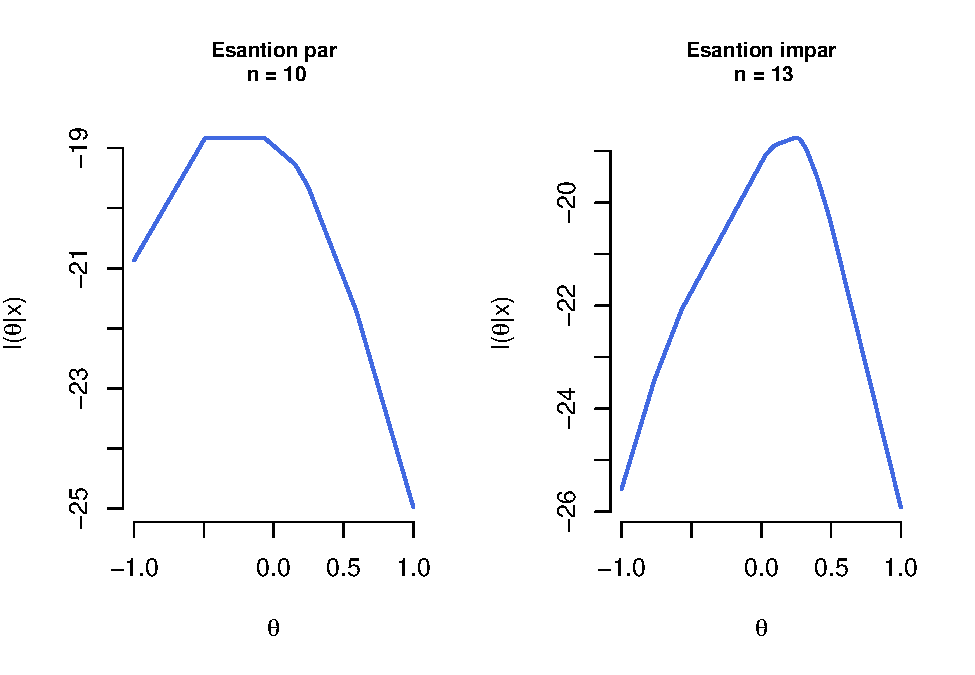
\includegraphics[width=0.7\linewidth]{Lab6_files/figure-latex/unnamed-chunk-14-1} \end{center}

\hypertarget{exemplu-de-evm-determinat-prin-soluux21bii-numerice}{%
\subsection{Exemplu de EVM determinat prin soluții
numerice}\label{exemplu-de-evm-determinat-prin-soluux21bii-numerice}}

\begin{rmdexercise}
Fie \(X_1,X_2,\ldots,X_n\) un eșantion de talie \(n\) dintr-o populație
logistică a cărei densitate este dată de formula

\[
  f_{\theta}(x) = \frac{e^{-(x-\theta)}}{\left(1+e^{-(x-\theta)}\right)^2}, \quad x\in\mathbb{R},\, \theta\in\mathbb{R} 
\]

Determinați estimatorul de verosimilitate maximă \(\hat{\theta}_n\)
pentru \(\theta\).
\end{rmdexercise}

Densitatea de repartiție și funcția de repartiție a repartiției
logistice sunt ilustrate mai jos (în R se folosesc funcțiile:
\texttt{rlogis}, \texttt{dlogis}, \texttt{plogis} și respectiv
\texttt{qlogis}):

\begin{Shaded}
\begin{Highlighting}[]
\CommentTok{# Generam graficele }
\NormalTok{pars =}\StringTok{ }\KeywordTok{c}\NormalTok{(}\DecValTok{2}\NormalTok{, }\DecValTok{4}\NormalTok{, }\DecValTok{6}\NormalTok{, }\DecValTok{9}\NormalTok{)}

\NormalTok{x =}\StringTok{ }\KeywordTok{seq}\NormalTok{(}\OperatorTok{-}\DecValTok{8}\NormalTok{, }\DecValTok{15}\NormalTok{, }\DataTypeTok{length.out =} \DecValTok{250}\NormalTok{)}

\KeywordTok{set.seed}\NormalTok{(}\DecValTok{1234}\NormalTok{)}
\NormalTok{cols =}\StringTok{ }\KeywordTok{sample}\NormalTok{(}\KeywordTok{colors}\NormalTok{(), }\KeywordTok{length}\NormalTok{(pars))}

\KeywordTok{par}\NormalTok{(}\DataTypeTok{mfrow =} \KeywordTok{c}\NormalTok{(}\DecValTok{1}\NormalTok{, }\DecValTok{2}\NormalTok{))}
\CommentTok{# densitatile}
\KeywordTok{plot}\NormalTok{(x, }\KeywordTok{dlogis}\NormalTok{(x, }\DataTypeTok{location =}\NormalTok{ pars[}\DecValTok{1}\NormalTok{]),}
     \DataTypeTok{xlab =} \StringTok{"x"}\NormalTok{,}
     \DataTypeTok{ylab =} \KeywordTok{TeX}\NormalTok{(}\StringTok{"$f_\{}\CharTok{\textbackslash{}\textbackslash{}}\StringTok{theta\}(x)$"}\NormalTok{),}
     \CommentTok{# ylim = c(0,1),}
     \DataTypeTok{col =} \StringTok{"brown3"}\NormalTok{, }
     \DataTypeTok{lwd =} \DecValTok{2}\NormalTok{, }\DataTypeTok{type =} \StringTok{"l"}\NormalTok{,}
     \DataTypeTok{bty =} \StringTok{"n"}\NormalTok{,}
     \DataTypeTok{main =} \StringTok{"Densitatea"}\NormalTok{)}

\ControlFlowTok{for}\NormalTok{ (i }\ControlFlowTok{in} \KeywordTok{seq}\NormalTok{(}\KeywordTok{length}\NormalTok{(pars)}\OperatorTok{-}\DecValTok{1}\NormalTok{))\{}
\NormalTok{  location =}\StringTok{ }\NormalTok{pars[i}\OperatorTok{+}\DecValTok{1}\NormalTok{]}
    
\NormalTok{  y =}\StringTok{ }\KeywordTok{dlogis}\NormalTok{(x, }\DataTypeTok{location =}\NormalTok{ location)}
  
  \KeywordTok{lines}\NormalTok{(x, y, }\DataTypeTok{lwd =} \DecValTok{2}\NormalTok{, }
        \DataTypeTok{col =}\NormalTok{ cols[i])}
\NormalTok{\}}

\KeywordTok{legend}\NormalTok{(}\StringTok{"topright"}\NormalTok{, }
       \DataTypeTok{legend =} \KeywordTok{TeX}\NormalTok{(}\KeywordTok{paste0}\NormalTok{(}\StringTok{"$}\CharTok{\textbackslash{}\textbackslash{}}\StringTok{theta = "}\NormalTok{, pars, }\StringTok{"$"}\NormalTok{)),}
       \DataTypeTok{col =}\NormalTok{ cols,}
       \DataTypeTok{lwd =} \KeywordTok{rep}\NormalTok{(}\DecValTok{2}\NormalTok{, }\KeywordTok{length}\NormalTok{(pars)),}
       \DataTypeTok{bty =} \StringTok{"n"}\NormalTok{,}
       \DataTypeTok{cex =} \FloatTok{0.7}\NormalTok{,}
       \DataTypeTok{seg.len =} \FloatTok{1.5}\NormalTok{)}

\CommentTok{# functiile de repartitie}
\KeywordTok{plot}\NormalTok{(x, }\KeywordTok{plogis}\NormalTok{(x, }\DataTypeTok{location =}\NormalTok{ pars[}\DecValTok{1}\NormalTok{]),}
     \DataTypeTok{xlab =} \StringTok{"x"}\NormalTok{,}
     \DataTypeTok{ylab =} \KeywordTok{TeX}\NormalTok{(}\StringTok{"$F_\{}\CharTok{\textbackslash{}\textbackslash{}}\StringTok{theta\}(x)$"}\NormalTok{),}
     \DataTypeTok{ylim =} \KeywordTok{c}\NormalTok{(}\DecValTok{0}\NormalTok{,}\DecValTok{1}\NormalTok{),}
     \DataTypeTok{col =} \StringTok{"brown3"}\NormalTok{, }
     \DataTypeTok{lwd =} \DecValTok{2}\NormalTok{, }\DataTypeTok{type =} \StringTok{"l"}\NormalTok{,}
     \DataTypeTok{bty =} \StringTok{"n"}\NormalTok{,}
     \DataTypeTok{main =} \StringTok{"Functia de repartitie"}\NormalTok{)}

\ControlFlowTok{for}\NormalTok{ (i }\ControlFlowTok{in} \KeywordTok{seq}\NormalTok{(}\KeywordTok{length}\NormalTok{(pars)}\OperatorTok{-}\DecValTok{1}\NormalTok{))\{}
\NormalTok{  location =}\StringTok{ }\NormalTok{pars[i}\OperatorTok{+}\DecValTok{1}\NormalTok{]}
  
\NormalTok{  y =}\StringTok{ }\KeywordTok{plogis}\NormalTok{(x, }\DataTypeTok{location =}\NormalTok{ location)}
  
  \KeywordTok{lines}\NormalTok{(x, y, }\DataTypeTok{lwd =} \DecValTok{2}\NormalTok{, }
        \DataTypeTok{col =}\NormalTok{ cols[i])}
\NormalTok{\}}

\KeywordTok{legend}\NormalTok{(}\StringTok{"bottomright"}\NormalTok{, }
       \DataTypeTok{legend =} \KeywordTok{TeX}\NormalTok{(}\KeywordTok{paste0}\NormalTok{(}\StringTok{"$}\CharTok{\textbackslash{}\textbackslash{}}\StringTok{theta = "}\NormalTok{, pars, }\StringTok{"$"}\NormalTok{)),}
       \DataTypeTok{col =}\NormalTok{ cols,}
       \DataTypeTok{lwd =} \KeywordTok{rep}\NormalTok{(}\DecValTok{2}\NormalTok{, }\KeywordTok{length}\NormalTok{(pars)),}
       \DataTypeTok{bty =} \StringTok{"n"}\NormalTok{,}
       \DataTypeTok{cex =} \FloatTok{0.7}\NormalTok{,}
       \DataTypeTok{seg.len =} \FloatTok{1.5}\NormalTok{)}
\end{Highlighting}
\end{Shaded}

\begin{center}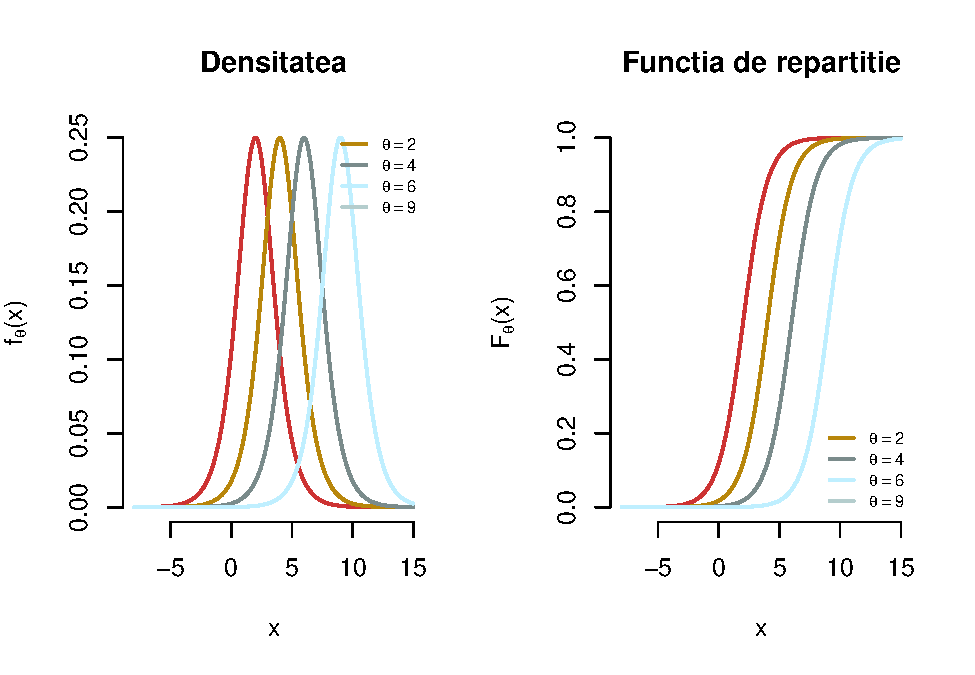
\includegraphics[width=0.7\linewidth]{Lab6_files/figure-latex/unnamed-chunk-16-1} \end{center}

Observăm că funcția de verosimilitate este dată de

\[
L(\theta|\mathbf{x}) = \prod_{i=1}^{n}f_{\theta}(x_i) = \prod_{i=1}^{n}\frac{e^{-(x_i-\theta)}}{\left(1+e^{-(x_i-\theta)}\right)^2}
\]

iar logaritmul funcției de verosimilitate este

\[
l(\theta|\mathbf{x}) = \sum_{i=1}^{n}\log{f_{\theta}(x_i)} = n\theta - n\bar{x}_n - 2\sum_{i=1}^{n}\log{\left(1+e^{-(x_i-\theta)}\right)}.
\]

Pentru a găsi valoarea lui \(\theta\) care maximizează logaritmul
funcției de verosimilitate și prin urmare a funcției de verosimilitate
trebuie să rezolvăm ecuația \(l'(\theta|\mathbf{x}) = 0\), unde derivata
lui \(l(\theta|\mathbf{x})\) este

\[
l'(\theta|\mathbf{x}) = n - 2\sum_{i = 1}^{n}\frac{e^{-(x_i-\theta)}}{1+e^{-(x_i-\theta)}}
\]

ceea ce conduce la ecuația

\[
  \sum_{i = 1}^{n}\frac{e^{-(x_i-\theta)}}{1+e^{-(x_i-\theta)}} = \frac{n}{2} \tag{$\star$}
\]

Chiar dacă această ecuație nu se simplifică, se poate arăta că această
ecuația admite soluție unică. Observăm că derivata parțiala a membrului
drept în (\(\star\)) devine

\[
\frac{\partial }{\partial \theta}\sum_{i = 1}^{n}\frac{e^{-(x_i-\theta)}}{1+e^{-(x_i-\theta)}} = \sum_{i = 1}^{n}\frac{e^{-(x_i-\theta)}}{\left(1+e^{-(x_i-\theta)}\right)^2}>0
\]

ceea ce arată că membrul stâng este o funcție strict crescătoare în
\(\theta\). Cum membrul stâng în (\(\star\)) tinde spre \(0\) atunci
când \(\theta\to-\infty\) și spre \(n\) pentru \(\theta\to\infty\)
deducem că ecuația (\(\star\)) admite soluție unică (vezi graficul de
mai jos).

\begin{Shaded}
\begin{Highlighting}[]
\KeywordTok{set.seed}\NormalTok{(}\DecValTok{112}\NormalTok{)}
\NormalTok{n =}\StringTok{ }\DecValTok{20}
\NormalTok{x =}\StringTok{ }\KeywordTok{rlogis}\NormalTok{(n, }\DataTypeTok{location =} \FloatTok{7.5}\NormalTok{)}

\CommentTok{# derivata logaritmului functiei de verosimilitate}
\NormalTok{dLogLogistic =}\StringTok{ }\ControlFlowTok{function}\NormalTok{(n, x, theta)\{}
  \KeywordTok{sapply}\NormalTok{(theta, }\ControlFlowTok{function}\NormalTok{(t)\{}
\NormalTok{    y =}\StringTok{ }\KeywordTok{exp}\NormalTok{(}\OperatorTok{-}\NormalTok{(x }\OperatorTok{-}\StringTok{ }\NormalTok{t))}
\NormalTok{    n }\OperatorTok{-}\StringTok{ }\DecValTok{2}\OperatorTok{*}\KeywordTok{sum}\NormalTok{(y}\OperatorTok{/}\NormalTok{(}\DecValTok{1}\OperatorTok{+}\NormalTok{y))}
\NormalTok{  \})}
\NormalTok{\}}

\NormalTok{theta =}\StringTok{ }\KeywordTok{seq}\NormalTok{(}\DecValTok{0}\NormalTok{, }\DecValTok{15}\NormalTok{, }\DataTypeTok{length.out =} \DecValTok{250}\NormalTok{)}

\NormalTok{mar.default <-}\StringTok{ }\KeywordTok{c}\NormalTok{(}\DecValTok{5}\NormalTok{,}\DecValTok{4}\NormalTok{,}\DecValTok{4}\NormalTok{,}\DecValTok{2}\NormalTok{) }\OperatorTok{+}\StringTok{ }\FloatTok{0.1}
\KeywordTok{par}\NormalTok{(}\DataTypeTok{mar =}\NormalTok{ mar.default }\OperatorTok{+}\StringTok{ }\KeywordTok{c}\NormalTok{(}\DecValTok{0}\NormalTok{, }\FloatTok{1.2}\NormalTok{, }\DecValTok{0}\NormalTok{, }\DecValTok{0}\NormalTok{))}

\KeywordTok{plot}\NormalTok{(theta, }\KeywordTok{dLogLogistic}\NormalTok{(n, x, theta), }\DataTypeTok{type =} \StringTok{"l"}\NormalTok{,}
     \DataTypeTok{col =} \StringTok{"royalblue"}\NormalTok{, }\DataTypeTok{lwd =} \DecValTok{2}\NormalTok{,}
     \DataTypeTok{bty =} \StringTok{"n"}\NormalTok{,}
     \DataTypeTok{xlab =} \KeywordTok{TeX}\NormalTok{(}\StringTok{"$}\CharTok{\textbackslash{}\textbackslash{}}\StringTok{theta$"}\NormalTok{),}
     \DataTypeTok{ylab =} \KeywordTok{TeX}\NormalTok{(}\StringTok{"$}\CharTok{\textbackslash{}\textbackslash{}}\StringTok{frac\{}\CharTok{\textbackslash{}\textbackslash{}}\StringTok{partial\}\{}\CharTok{\textbackslash{}\textbackslash{}}\StringTok{partial }\CharTok{\textbackslash{}\textbackslash{}}\StringTok{theta\} l(}\CharTok{\textbackslash{}\textbackslash{}}\StringTok{theta | x)$"}\NormalTok{))}

\KeywordTok{abline}\NormalTok{(}\DataTypeTok{h =} \DecValTok{0}\NormalTok{, }\DataTypeTok{col =} \StringTok{"brown3"}\NormalTok{,}
       \DataTypeTok{lty =} \DecValTok{2}\NormalTok{)}
\end{Highlighting}
\end{Shaded}

\begin{center}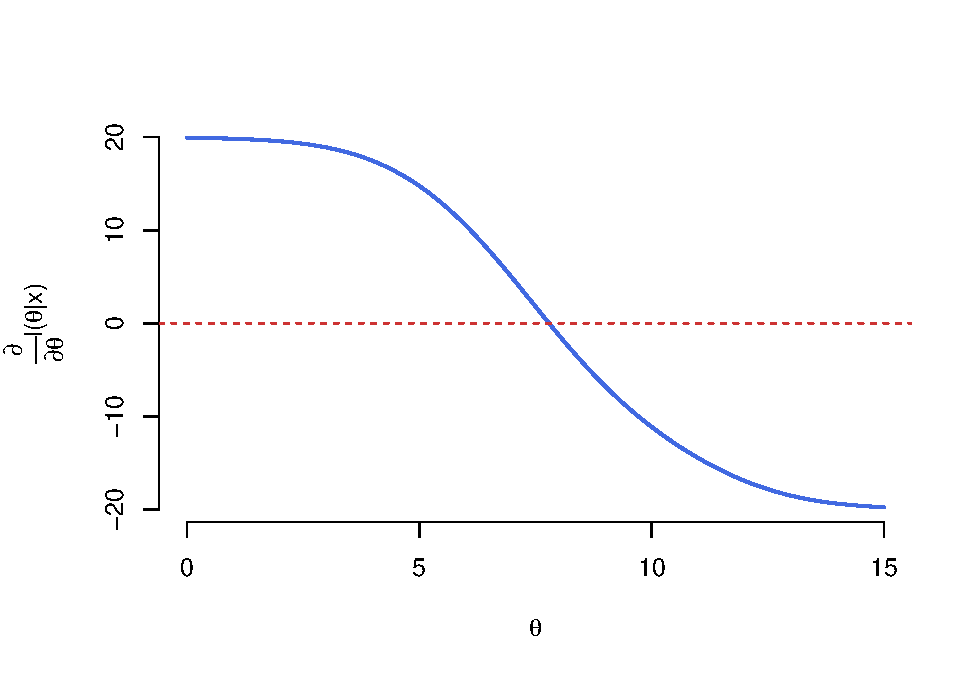
\includegraphics[width=0.7\linewidth]{Lab6_files/figure-latex/unnamed-chunk-17-1} \end{center}

Cum nu putem găsi o soluție a ecuației \(l'(\theta|\mathbb{x}) = 0\) sub
formă compactă, este necesar să apelăm la metode numerice. O astfel de
metodă numerică este binecunoscuta
\href{https://en.wikipedia.org/wiki/Newton\%27s_method}{metodă a lui
Newton-Raphson}. Metoda presupune să începem cu o valoare (soluție)
inițială \(\hat{\theta}^{(0)}\) și să alegem, plecând de la aceasta, o
nouă valoare \(\hat{\theta}^{(1)}\) definită prin

\[
  \hat{\theta}^{(1)} = \hat{\theta}^{(0)} - \frac{l'\left(\hat{\theta}^{(0)}\right)}{l''\left(\hat{\theta}^{(0)}\right)},
\]

adică \(\hat{\theta}^{(1)}\) este intersecția cu axa absciselor a
tangentei în punctul
\(\left(\hat{\theta}^{(0)}, l'\left(\hat{\theta}^{(0)}\right)\right)\)
la graficul funcției \(l'(\theta)\). Ideea este de a itera procesul până
când soluția converge, cu alte cuvinte pornind de la o valoare
\emph{rezonabilă} de start \(\hat{\theta}^{(0)}\) la pasul \(k+1\) avem

\[
  \hat{\theta}^{(k+1)} = \hat{\theta}^{(k)} - \frac{l'\left(\hat{\theta}^{(k)}\right)}{l''\left(\hat{\theta}^{(k)}\right)}
\]

și oprim procesul atunco când \(k\) este suficient de mare și/sau
\(\left|\hat{\theta}^{(k+1)} - \hat{\theta}^{(k)}\right|\) este
suficient de mic. Următorul grafic ilustrează grafic algoritmul lui
Newton:

\begin{Shaded}
\begin{Highlighting}[]
\KeywordTok{set.seed}\NormalTok{(}\DecValTok{112}\NormalTok{)}
\NormalTok{n =}\StringTok{ }\DecValTok{20}
\NormalTok{x =}\StringTok{ }\KeywordTok{rlogis}\NormalTok{(n, }\DataTypeTok{location =} \FloatTok{7.5}\NormalTok{)}

\CommentTok{# derivata logaritmului functiei de verosimilitate}
\NormalTok{dLogLogistic =}\StringTok{ }\ControlFlowTok{function}\NormalTok{(n, x, theta)\{}
  \KeywordTok{sapply}\NormalTok{(theta, }\ControlFlowTok{function}\NormalTok{(t)\{}
\NormalTok{    y =}\StringTok{ }\KeywordTok{exp}\NormalTok{(}\OperatorTok{-}\NormalTok{(x }\OperatorTok{-}\StringTok{ }\NormalTok{t))}
\NormalTok{    n }\OperatorTok{-}\StringTok{ }\DecValTok{2}\OperatorTok{*}\KeywordTok{sum}\NormalTok{(y}\OperatorTok{/}\NormalTok{(}\DecValTok{1}\OperatorTok{+}\NormalTok{y))}
\NormalTok{  \})}
\NormalTok{\}}

\NormalTok{theta =}\StringTok{ }\KeywordTok{seq}\NormalTok{(}\DecValTok{0}\NormalTok{, }\DecValTok{15}\NormalTok{, }\DataTypeTok{length.out =} \DecValTok{250}\NormalTok{)}

\NormalTok{mar.default <-}\StringTok{ }\KeywordTok{c}\NormalTok{(}\DecValTok{5}\NormalTok{,}\DecValTok{4}\NormalTok{,}\DecValTok{4}\NormalTok{,}\DecValTok{2}\NormalTok{) }\OperatorTok{+}\StringTok{ }\FloatTok{0.1}
\KeywordTok{par}\NormalTok{(}\DataTypeTok{mar =}\NormalTok{ mar.default }\OperatorTok{+}\StringTok{ }\KeywordTok{c}\NormalTok{(}\DecValTok{0}\NormalTok{, }\FloatTok{1.2}\NormalTok{, }\DecValTok{0}\NormalTok{, }\DecValTok{0}\NormalTok{))}

\KeywordTok{plot}\NormalTok{(theta, }\KeywordTok{dLogLogistic}\NormalTok{(n, x, theta), }\DataTypeTok{type =} \StringTok{"l"}\NormalTok{,}
     \DataTypeTok{col =} \StringTok{"royalblue"}\NormalTok{, }\DataTypeTok{lwd =} \DecValTok{2}\NormalTok{,}
     \DataTypeTok{bty =} \StringTok{"n"}\NormalTok{,}
     \DataTypeTok{xlab =} \KeywordTok{TeX}\NormalTok{(}\StringTok{"$}\CharTok{\textbackslash{}\textbackslash{}}\StringTok{theta$"}\NormalTok{),}
     \DataTypeTok{ylab =} \KeywordTok{TeX}\NormalTok{(}\StringTok{"$}\CharTok{\textbackslash{}\textbackslash{}}\StringTok{frac\{}\CharTok{\textbackslash{}\textbackslash{}}\StringTok{partial\}\{}\CharTok{\textbackslash{}\textbackslash{}}\StringTok{partial }\CharTok{\textbackslash{}\textbackslash{}}\StringTok{theta\} l(}\CharTok{\textbackslash{}\textbackslash{}}\StringTok{theta | x)$"}\NormalTok{))}

\KeywordTok{abline}\NormalTok{(}\DataTypeTok{h =} \DecValTok{0}\NormalTok{, }\DataTypeTok{col =} \StringTok{"brown3"}\NormalTok{,}
       \DataTypeTok{lty =} \DecValTok{2}\NormalTok{)}

\CommentTok{# ilustrarea metodei Newton}

\NormalTok{dl =}\StringTok{ }\ControlFlowTok{function}\NormalTok{(theta) n }\OperatorTok{-}\StringTok{ }\DecValTok{2} \OperatorTok{*}\StringTok{ }\KeywordTok{sum}\NormalTok{(}\KeywordTok{exp}\NormalTok{(theta }\OperatorTok{-}\StringTok{ }\NormalTok{x) }\OperatorTok{/}\StringTok{ }\NormalTok{(}\DecValTok{1} \OperatorTok{+}\StringTok{ }\KeywordTok{exp}\NormalTok{(theta }\OperatorTok{-}\StringTok{ }\NormalTok{x)))}
\NormalTok{ddl =}\StringTok{ }\ControlFlowTok{function}\NormalTok{(theta) \{}\OperatorTok{-}\DecValTok{2} \OperatorTok{*}\StringTok{ }\KeywordTok{sum}\NormalTok{(}\KeywordTok{exp}\NormalTok{(theta }\OperatorTok{-}\StringTok{ }\NormalTok{x) }\OperatorTok{/}\StringTok{ }\NormalTok{(}\DecValTok{1} \OperatorTok{+}\StringTok{ }\KeywordTok{exp}\NormalTok{(theta }\OperatorTok{-}\StringTok{ }\NormalTok{x))}\OperatorTok{^}\DecValTok{2}\NormalTok{)\}}

\NormalTok{x0 =}\StringTok{ }\DecValTok{5} \CommentTok{# punctul de start}

\KeywordTok{points}\NormalTok{(x0, }\DecValTok{0}\NormalTok{, }\DataTypeTok{pch =} \DecValTok{16}\NormalTok{, }\DataTypeTok{col =} \StringTok{"black"}\NormalTok{)}
\KeywordTok{text}\NormalTok{(x0, }\DecValTok{0}\NormalTok{, }\DataTypeTok{labels =} \KeywordTok{TeX}\NormalTok{(}\StringTok{"$}\CharTok{\textbackslash{}\textbackslash{}}\StringTok{hat\{}\CharTok{\textbackslash{}\textbackslash{}}\StringTok{theta\}^\{(0)\}$"}\NormalTok{), }\DataTypeTok{pos =} \DecValTok{1}\NormalTok{, }\DataTypeTok{cex =} \FloatTok{0.8}\NormalTok{)}
\KeywordTok{segments}\NormalTok{(x0, }\DecValTok{0}\NormalTok{, x0, }\KeywordTok{dl}\NormalTok{(x0), }\DataTypeTok{lty =} \DecValTok{2}\NormalTok{, }\DataTypeTok{col =} \StringTok{"grey50"}\NormalTok{)}
\KeywordTok{points}\NormalTok{(x0, }\KeywordTok{dl}\NormalTok{(x0), }\DataTypeTok{pch =} \DecValTok{4}\NormalTok{)}

\NormalTok{x1 =}\StringTok{ }\NormalTok{x0 }\OperatorTok{-}\StringTok{ }\KeywordTok{dl}\NormalTok{(x0)}\OperatorTok{/}\KeywordTok{ddl}\NormalTok{(x0)}

\KeywordTok{segments}\NormalTok{(x0, }\KeywordTok{dl}\NormalTok{(x0), x1, }\DecValTok{0}\NormalTok{, }\DataTypeTok{lty =} \DecValTok{1}\NormalTok{, }\DataTypeTok{lwd =} \DecValTok{2}\NormalTok{, }\DataTypeTok{col =} \StringTok{"grey50"}\NormalTok{)}
\KeywordTok{points}\NormalTok{(x1, }\DecValTok{0}\NormalTok{, }\DataTypeTok{pch =} \DecValTok{16}\NormalTok{, }\DataTypeTok{col =} \StringTok{"black"}\NormalTok{)}
\KeywordTok{text}\NormalTok{(x1, }\DecValTok{0}\NormalTok{, }\DataTypeTok{labels =} \KeywordTok{TeX}\NormalTok{(}\StringTok{"$}\CharTok{\textbackslash{}\textbackslash{}}\StringTok{hat\{}\CharTok{\textbackslash{}\textbackslash{}}\StringTok{theta\}^\{(1)\}$"}\NormalTok{), }\DataTypeTok{pos =} \DecValTok{1}\NormalTok{, }\DataTypeTok{cex =} \FloatTok{0.8}\NormalTok{)}
\KeywordTok{segments}\NormalTok{(x1, }\DecValTok{0}\NormalTok{, x1, }\KeywordTok{dl}\NormalTok{(x1), }\DataTypeTok{lty =} \DecValTok{2}\NormalTok{, }\DataTypeTok{col =} \StringTok{"grey50"}\NormalTok{)}
\KeywordTok{points}\NormalTok{(x1, }\KeywordTok{dl}\NormalTok{(x1), }\DataTypeTok{pch =} \DecValTok{4}\NormalTok{)}

\NormalTok{x2 =}\StringTok{ }\NormalTok{x1 }\OperatorTok{-}\StringTok{ }\KeywordTok{dl}\NormalTok{(x1)}\OperatorTok{/}\KeywordTok{ddl}\NormalTok{(x1)}

\KeywordTok{segments}\NormalTok{(x1, }\KeywordTok{dl}\NormalTok{(x1), x2, }\DecValTok{0}\NormalTok{, }\DataTypeTok{lty =} \DecValTok{1}\NormalTok{, }\DataTypeTok{lwd =} \DecValTok{2}\NormalTok{, }\DataTypeTok{col =} \StringTok{"grey50"}\NormalTok{)}
\KeywordTok{points}\NormalTok{(x2, }\DecValTok{0}\NormalTok{, }\DataTypeTok{pch =} \DecValTok{16}\NormalTok{, }\DataTypeTok{col =} \StringTok{"black"}\NormalTok{)}
\KeywordTok{text}\NormalTok{(x2, }\DecValTok{0}\NormalTok{, }\DataTypeTok{labels =} \KeywordTok{TeX}\NormalTok{(}\StringTok{"$}\CharTok{\textbackslash{}\textbackslash{}}\StringTok{hat\{}\CharTok{\textbackslash{}\textbackslash{}}\StringTok{theta\}^\{(2)\}$"}\NormalTok{), }\DataTypeTok{pos =} \DecValTok{1}\NormalTok{, }\DataTypeTok{cex =} \FloatTok{0.8}\NormalTok{)}
\end{Highlighting}
\end{Shaded}

\begin{center}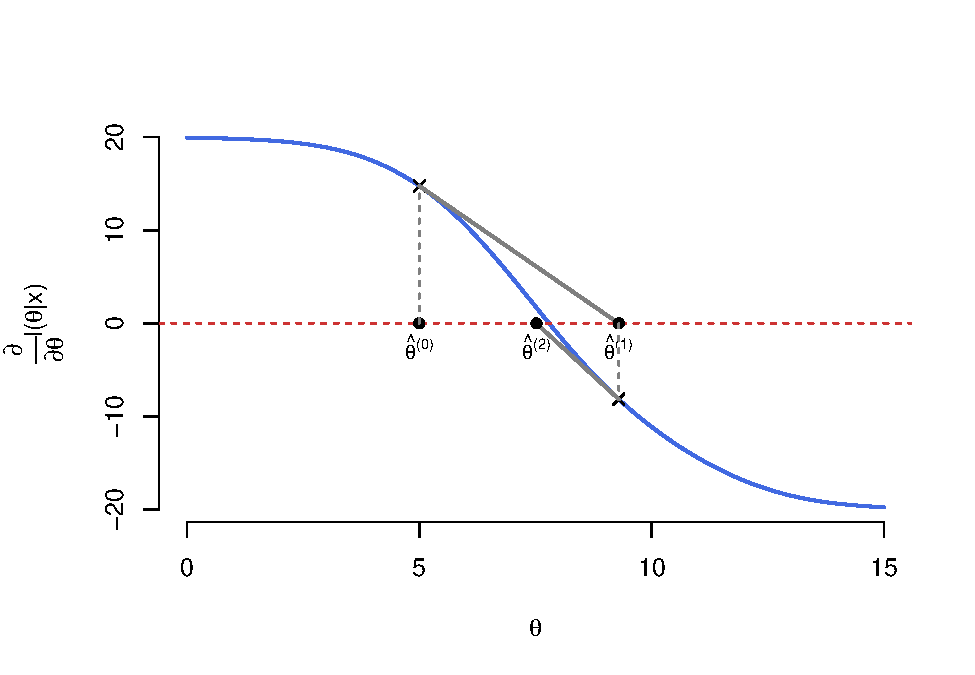
\includegraphics[width=0.7\linewidth]{Lab6_files/figure-latex/unnamed-chunk-18-1} \end{center}

\textbf{Obs:} Singurul lucru care se schimbă atunci când trecem de la
scalar la vector, este funcția \(l(\theta)\) care acum este o funcție de
\(p>1\) variabile,
\(\theta = (\theta_1, \theta_2, \ldots, \theta_p)^{\intercal}\in\mathbb{R}^p\).
În acest context \(l'(\theta)\) este un vector de derivate parțiale iar
\(l''(\theta)\) este o matrice de derivate parțiale de ordin doi. Prin
urmare itarațiile din metoda lui Newton sunt

\[
  \hat{\theta}^{(k+1)} = \hat{\theta}^{(k)} - \left[l''\left(\hat{\theta}^{(k)}\right)\right]^{-1}l'\left(\hat{\theta}^{(k)}\right)
\] unde \([\cdot]^{-1}\) este
\href{https://en.wikipedia.org/wiki/Moore\%E2\%80\%93Penrose_inverse}{pseudoinversa}
unei matrici.

Funcția de mai jos implementează metoada lui Newton pentru cazul
multidimensional:

\begin{Shaded}
\begin{Highlighting}[]
\CommentTok{# Metoda lui Newton}

\NormalTok{newton <-}\StringTok{ }\ControlFlowTok{function}\NormalTok{(f, df, x0, }\DataTypeTok{eps=}\FloatTok{1e-08}\NormalTok{, }\DataTypeTok{maxiter=}\DecValTok{1000}\NormalTok{, ...) \{}
  \CommentTok{# in caz ca nu e incarcat pachetul sa putem accesa pseudoinversa}
  \ControlFlowTok{if}\NormalTok{(}\OperatorTok{!}\KeywordTok{exists}\NormalTok{(}\StringTok{"ginv"}\NormalTok{)) }\KeywordTok{library}\NormalTok{(MASS) }
  
\NormalTok{  x <-}\StringTok{ }\NormalTok{x0}
\NormalTok{  k <-}\StringTok{ }\DecValTok{0}
  
  \ControlFlowTok{repeat}\NormalTok{ \{}
\NormalTok{    k <-}\StringTok{ }\NormalTok{k }\OperatorTok{+}\StringTok{ }\DecValTok{1}
    
\NormalTok{    x.new <-}\StringTok{ }\NormalTok{x }\OperatorTok{-}\StringTok{ }\KeywordTok{as.numeric}\NormalTok{(}\KeywordTok{ginv}\NormalTok{(}\KeywordTok{df}\NormalTok{(x, ...)) }\OperatorTok\StringTok{ }\KeywordTok{f}\NormalTok{(x, ...))}
    
    \ControlFlowTok{if}\NormalTok{(}\KeywordTok{mean}\NormalTok{(}\KeywordTok{abs}\NormalTok{(x.new }\OperatorTok{-}\StringTok{ }\NormalTok{x)) }\OperatorTok{<}\StringTok{ }\NormalTok{eps }\OperatorTok{|}\StringTok{ }\NormalTok{k }\OperatorTok{>=}\StringTok{ }\NormalTok{maxiter) \{}
      \ControlFlowTok{if}\NormalTok{(k }\OperatorTok{>=}\StringTok{ }\NormalTok{maxiter) }\KeywordTok{warning}\NormalTok{(}\StringTok{"S-a atins numarul maxim de iteratii!"}\NormalTok{)}
      \ControlFlowTok{break}
\NormalTok{    \}}
\NormalTok{    x <-}\StringTok{ }\NormalTok{x.new}
\NormalTok{  \}}
\NormalTok{  out <-}\StringTok{ }\KeywordTok{list}\NormalTok{(}\DataTypeTok{solution =}\NormalTok{ x.new, }\DataTypeTok{value =} \KeywordTok{f}\NormalTok{(x.new, ...), }\DataTypeTok{iter =}\NormalTok{ k)}
  
  \KeywordTok{return}\NormalTok{(out)}
\NormalTok{\}}
\end{Highlighting}
\end{Shaded}

Să presupunem că am observat următorul eșantion de talie \(20\) din
repartiția logistică:

\begin{verbatim}
 [1]  6.996304  9.970107 12.304991 11.259549  6.326912  5.378941  4.299639
 [8]  8.484635  5.601117  7.094335  6.324731  6.868456  9.753360  8.042095
[15]  8.227830 10.977982  7.743096  7.722159  8.562884  6.968356
\end{verbatim}

\begin{Shaded}
\begin{Highlighting}[]
\KeywordTok{set.seed}\NormalTok{(}\DecValTok{112}\NormalTok{)}
\NormalTok{x =}\StringTok{ }\KeywordTok{rlogis}\NormalTok{(}\DecValTok{20}\NormalTok{, }\DataTypeTok{location =} \FloatTok{7.5}\NormalTok{)}

\NormalTok{n =}\StringTok{ }\KeywordTok{length}\NormalTok{(x)}
\NormalTok{dl =}\StringTok{ }\ControlFlowTok{function}\NormalTok{(theta) n }\OperatorTok{-}\StringTok{ }\DecValTok{2} \OperatorTok{*}\StringTok{ }\KeywordTok{sum}\NormalTok{(}\KeywordTok{exp}\NormalTok{(theta }\OperatorTok{-}\StringTok{ }\NormalTok{x) }\OperatorTok{/}\StringTok{ }\NormalTok{(}\DecValTok{1} \OperatorTok{+}\StringTok{ }\KeywordTok{exp}\NormalTok{(theta }\OperatorTok{-}\StringTok{ }\NormalTok{x)))}
\NormalTok{ddl =}\StringTok{ }\ControlFlowTok{function}\NormalTok{(theta) \{}\OperatorTok{-}\DecValTok{2} \OperatorTok{*}\StringTok{ }\KeywordTok{sum}\NormalTok{(}\KeywordTok{exp}\NormalTok{(theta }\OperatorTok{-}\StringTok{ }\NormalTok{x) }\OperatorTok{/}\StringTok{ }\NormalTok{(}\DecValTok{1} \OperatorTok{+}\StringTok{ }\KeywordTok{exp}\NormalTok{(theta }\OperatorTok{-}\StringTok{ }\NormalTok{x))}\OperatorTok{^}\DecValTok{2}\NormalTok{)\}}

\NormalTok{logis.newton =}\StringTok{ }\KeywordTok{newton}\NormalTok{(dl, ddl, }\KeywordTok{median}\NormalTok{(x))}
\end{Highlighting}
\end{Shaded}

și aplicănd metoda lui Newton găsim estimatorul de verosimilitate maximă
\(\hat{\theta}_n=\) 7.7933 după numai 3 iterații (datele au fost
simulate folosin \(\theta = 7.5\)).

\end{document}
